\documentclass[aps,showpacs,%twocolumn,
prd,superscriptaddress,nofootinbib]{revtex4}

\usepackage{amsmath}
\usepackage{amsfonts}
\usepackage{amssymb}
\usepackage{latexsym}
\usepackage{graphicx}
\usepackage{bm}
\usepackage{color}
\usepackage{enumerate}
\usepackage{ulem}

\usepackage{graphicx}
\usepackage[caption=false]{subfig}
%\usepackage{caption}
%\usepackage{subcaption}
%\captionsetup{compatibility=false}

\newcommand{\be}{\begin{equation}}
\newcommand{\ee}{\end{equation}}
\newcommand\ud{{\mathrm{d}}}
\newcommand\uD{{\mathrm{D}}}
\newcommand\calO{{\mathcal{O}}}
\newcommand\calM{{\mathcal{M}}}
\newcommand\calF{{\mathcal{F}}}
\newcommand\calT{{\mathcal{T}}}
\newcommand\bfx{\mathbf{x}}
\newcommand{\ov}[1]{\overline{#1}}
\newcommand{\ph}[1]{\phantom{#1}}
\newcommand{\cte}{\mathrm{cte}}
\newcommand{\nn}{\nonumber}
\newcommand{\hatk}{\hat{k}}
\newcommand{\Hz}{\,\mathrm{Hz}}
\newcommand{\sinc}{\,\mathrm{sinc}}
\newcommand{\Msol}{M_{\odot}}
\newcommand{\tf}{t_{f}}
\newcommand{\Tf}{T_{f}}
\newcommand{\tfd}{t_{f}^{d}}

\begin{document}

\title{Modulations and delays in Fourier domain: precessing binaries and LISA-type detector response}

\author{A. A. Author}
\affiliation{U. U. University}

%\author{John G. Baker}
%\affiliation{Gravitational Astrophysics Laboratory, NASA Goddard Space Flight Center, 8800 Greenbelt Rd., Greenbelt, MD 20771, USA}
%\author{Alessandra Buonanno}
%\affiliation{Department of Physics, University of Maryland, College Park, MD 20742, USA}
%\affiliation{Max Planck Institute for Gravitational Physics (Albert Einstein Institute), Am M\"uhlenberg 1, Potsdam-Golm, 14476, Germany}
%\author{Philip. B. Graff}
%\affiliation{Department of Physics, University of Maryland, College Park, MD 20742, USA}
%\affiliation{Gravitational Astrophysics Laboratory, NASA Goddard Space Flight Center, 8800 Greenbelt Rd., Greenbelt, MD 20771, USA}
%\author{Sylvain Marsat}
%\affiliation{Max Planck Institute for Gravitational Physics (Albert Einstein Institute), Am M\"uhlenberg 1, Potsdam-Golm, 14476, Germany}


\date{\today}

\begin{abstract}

[Abstract]

\end{abstract}

\pacs{
04.25.D-, % numerical relativity
04.70.Bw, % classical black holes
04.80.Nn, % Gravitational wave detectors and experiments
95.30.Sf, % relativity and gravitation
95.55.Ym, % Gravitational radiation detectors
97.60.Lf  % black holes (astrophysics)
}

\maketitle

%%%%%%%%%%%%%%%%%%%%%%%%%%%%%%%%%%%%
%%%%%%%%%%%%%%%%%%%%%%%%%%%%%%%%%%%%

\section{Introduction}
\label{sec:intro}

[Introduction]



%%%%%%%%%%%%%%%%%%%%%%%%%%%%%%%%%%%%
%%%%%%%%%%%%%%%%%%%%%%%%%%%%%%%%%%%%

\section{Fourier-domain waveforms and separation of timescales}
\label{sec:motivation}

%%%%%%%%%%%%%%%%%%%%%%%%%%%%%%%%%%%%

\subsection{Waveforms in the Fourier domain and stationary phase approximation}
\label{subsec:SPA}

The convention we will be using for the Fourier transform of a signal $h(t)$ is
\be\label{eq:defFT}
	\tilde{h}(f) =  \int \ud t \, e^{+2i\pi f t} h(t) \,.
\ee
Notice that this sign convention is not the most frequently used in the literature. We chose it to ensure that, with the conventions of~\cite{BlanchetLiving}, spin-weighted spherical modes $h_{\ell m}$ with $m>0$ will have support mostly for positive frequencies. One can revert to the more usual convention by taking $f\rightarrow -f$.

The gravitational waveform emitted in the direction $(\Theta, \Phi)$, with its two polarizations $h_{+},h_{\times}$, can be decomposed in spin-weighted spherical modes as~\cite{Thorne80}
\be\label{eq:defmodes}
	h_{+} - i h_{\times} = \sum\limits_{\ell \geq 2} \sum\limits_{m=-\ell}^{+\ell} {}_{-2}Y_{\ell m}(\Theta,\Phi) h_{\ell m} \,,
\ee
where the ${}_{-2}Y_{\ell m}(\Theta,\Phi)$ are spin-weighted spherical harmonics. Since we will work in the Fourier domain, it will be useful to write the contributions of the individual modes to the Fourier transforms of the polarizations as
\begin{subequations}\label{eq:hpcfrommodes}
\begin{align}
	\tilde{h}_{+}(f) &= \frac{1}{2} \sum\limits_{\ell \geq 2} \sum\limits_{m=-\ell}^{+\ell} \left( {}_{-2}Y_{\ell m} \widetilde{h_{\ell m}}(f) + {}_{-2}Y_{\ell m}^{*} \widetilde{h_{\ell m}}(-f)^{*} \right) \,, \\
	\tilde{h}_{\times}(f) &= \frac{i}{2} \sum\limits_{\ell \geq 2} \sum\limits_{m=-\ell}^{+\ell} \left( {}_{-2}Y_{\ell m} \widetilde{h_{\ell m}}(f) - {}_{-2}Y_{\ell m}^{*} \widetilde{h_{\ell m}}(-f)^{*} \right) \,,
\end{align}
\end{subequations}
where we used $\widetilde{h_{\ell m}^{*}}(f) = \widetilde{h_{\ell m}}(-f)^{*}$. In the following, we will denote generically by $h$ an individual mode of the waveform, dropping the mode indices $\ell m$, and we will often refer to the Fourier-domain amplitude $A$ and phase $\Psi$ of the mode, according to
\be
	\tilde{h}(f) \equiv A(f) e^{-i\Psi(f)} \,.
\ee
Since we intend to work in the Fourier domain, we will use PhenomD waveforms~\cite{Khan+15}. These phenomenological waveforms provide analytic fits for both the Fourier-domain amplitude and phase of the 22 mode, with fit coefficients that were calibrated on EOB/NR hybrids [describe smoothing across intervals]. Fig.~\ref{fig:ampphase} shows an example of amplitude and phase in geometric units for an equal-mass binary.

\begin{figure}
  \centering
  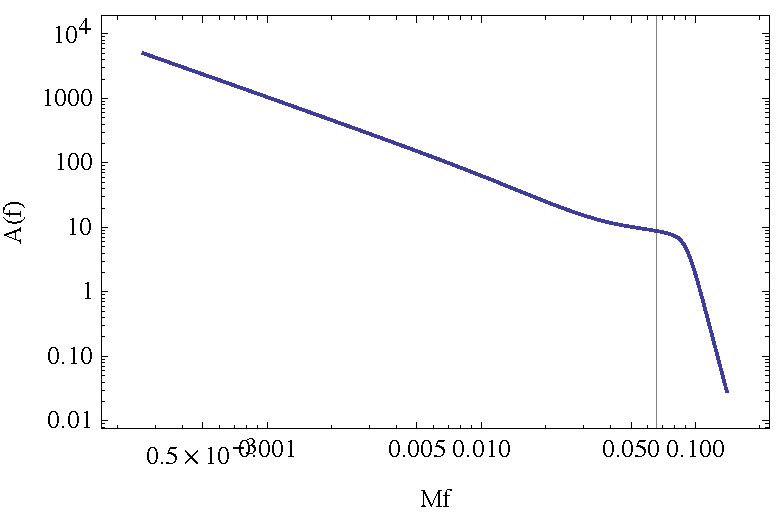
\includegraphics[width=.48\linewidth]{plots/Af.pdf}
  \hspace{0.2cm}
  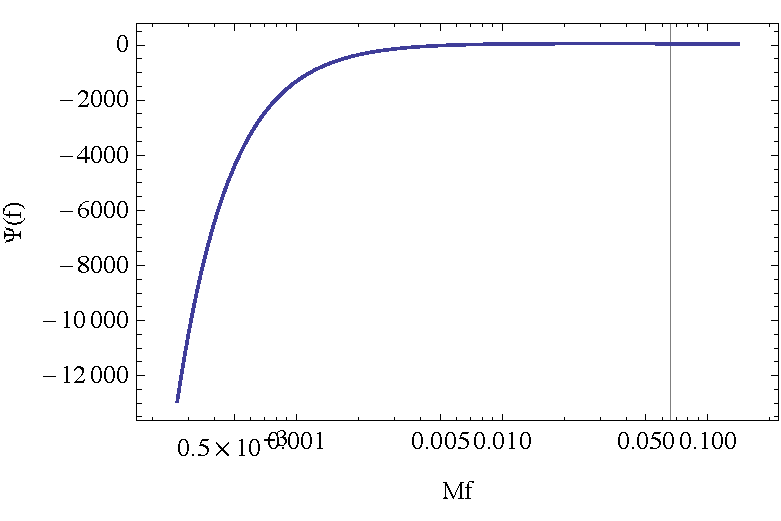
\includegraphics[width=.48\linewidth]{plots/Psif.pdf}
  \caption{Fourier-domain amplitude and phase in geometric units for an equal-mass, non-spinning system. The vertical line represents $\omega_{22}^{\rm peak}/2\pi$, the frequency corresponding to the time-domain frequency of the waveform at the peak amplitude. The starting frequency $Mf_{min} = 2.6\times 10^{-4}$ is appropriate for a 2-years observation of a $M=10^{6} M_{\odot}$ system by LISA, or for an observation by LIGO/Virgo of a $M=5.4 M_{\odot}$ system entering the instrument band at $10\Hz$.}
  \label{fig:ampphase}
\end{figure}

We recall that, with our sign convention, the effect of a positive shift in time $h_{\Delta t} (t) = h(t- \Delta t)$ is
\be
	\tilde{h}_{\Delta t}(f) = e^{2i\pi f \Delta t} \tilde{h}(f) \,.
\ee
If we also allow for a global shift in phase of the signal, which corresponds to a rotation of the unit vector pointing towards the observer in the frame of the gravitational waves source, a constant term can also be added (note that the effect of such a rotation gives different phase changes $e^{\pm i m \delta \phi}$ for the different modes of the radiation). We see that both a constant and a linear term in the Fourier-domain phase can be adjusted by changing extrinsic parameters. Thus, as is well known, apart from the relative phases of the modes for waveforms that include higher harmonics, the intrinsic information on the phasing is contained in the second derivative of the Fourier-domain phase $\Psi(f)$.

We recall below an approximation widely used to model gravitational waves signals emitted by inspiralling binaries, the stationary phase approximation (thereafter SPA). It applies in general to chirping signals, and we refer the reader to~\ref{} for details. One first writes the time-domain signal in amplitude and phase form as $h(t) = a(t) e^{-2i\varphi(t)}$, where for gravitational wave signals $\varphi$ will correspond to the orbital phase, with the orbital frequency being $\omega = \dot{\varphi}$. In order to keep close to the notations used in the gravitational wave literature, we introduced a factor of 2 in the phase of the wave, which is appropriate for the dominant 22 harmonic of the signal. The approximation then applies to signals verifying the conditions
%
\be\label{eq:conditionSPA}
	\left| \frac{\dot{a}/a}{\omega} \right| \ll 1\,, \quad \left|\frac{\dot{\omega}}{\omega^{2}} \right| \ll 1\,, \quad \left| \frac{(\dot{a}/a)^{2}}{\dot{\omega}} \right| \ll 1 \,.
\ee
%
Since the integral~\eqref{eq:defFT} defining the Fourier transform is rapidly oscillatory unless the term $2\pi f t$ cancels the evolution of $-2\varphi(t)$, its support is well centered around the point of stationary phase. This determines the time-to-frequency correspondence in the stationary phase approximation, and leads to the definition of this time as an implicit function of frequency by the relation
%
\be\label{eq:deftfSPA}
	\omega(t_{f}^{\rm SPA}) = \pi  f \,.
\ee
% 
For a chirping signal of increasing phase, $\omega>0$ and $\dot{\omega}>0$, there is a unique point of stationary phase, located in the positive frequency range $f>0$. Using the conditions above, one can formally expand the signal around $t_{f}^{\rm SPA}$ to quadratic order in time, according to
\be
	\tilde{h}_{\rm SPA} (f) \simeq a(t_{f}^{\rm SPA}) \exp\left[2i\pi f t_{f}^{\rm SPA}-2i\varphi(t_{f}^{\rm SPA}) \right]  \int \ud t \, e^{-i \dot{\omega} (t_{f}^{\rm SPA}) (t-t_{f}^{\rm SPA})^{2}} \,.
\ee
Note that to be able to treat the amplitude as a constant in the integral above, we used the third condition in~\eqref{eq:conditionSPA}. The resulting complex Gaussian integral yields\footnote{Note that the expressions given here are valid for the $22$ mode of the waveform.}
\begin{subequations}
\begin{align}
	\tilde{h}_{\rm SPA}(f) &= A_{\rm SPA}(f) e^{-i\Psi_{\rm SPA}(f)} \,, \\
	A_{\rm SPA}(f) &= a(t_{f}^{\rm SPA}) \sqrt{\frac{\pi}{\dot{\omega}(t_{f}^{\rm SPA})}} \,, \\
	\Psi_{\rm SPA}(f) &= 2\varphi(t_{f}^{\rm SPA}) - 2\pi f t_{f}^{\rm SPA} + \frac{\pi}{4} \,.
\end{align}
\end{subequations}
Ref.~\cite{Droz+99} evaluated the first correction to this approximation, within the context of post-Newtonian signals, and found that it can be considered as a term of the fifth post-Newtonian order, beyond the accuracy level of our current best models~\cite{BlanchetLiving}.

To understand the separation of timescales in the problem, it will be useful to have at hand the leading-order scaling laws for an inspiral (at the Newtonian order in the PN language). Although inaccurate for the purpose of waveform modelling, these Newtonian estimates will give a good qualitative description of the order of magnitude of the relevant timescales in the inspiral. For a binary with masses $m_{1}, m_{2}$, we define the total mass $m=m_{1}+m_{2}$ and the symmetric mass ratio $\nu = m_{1}m_{2}/m^{2}$. Introducing a time of coalescence $t_{c}$, the relations between the orbital frequency and phase and the time to coalescence $t_{c} - t$ are then given by
\begin{subequations}
\begin{align}
	\omega(t) &= \left[ \frac{256\nu}{5c^{5}} (Gm)^{5/3} (t_{c}-t) \right]^{-3/8} \,, \\
	\varphi(t) &= -\left[ \frac{c^{3}}{G m \nu^{3/5}} (t_{c}-t) \right]^{5/8} \,.
\end{align}
\end{subequations}
For this Newtonian inspiral, applying the SPA gives for the $22$ mode $\tilde{h}(f) = A_{\rm N}(f)e^{-i\Psi_{\rm N}(f)}$ with
%
\begin{subequations}
\begin{align}
	A_{N}(f) &= \frac{G^{2}m^{2} \pi}{Dc^{5}} \sqrt{\frac{2\nu}{3}} v^{-7/2}\,,\\
	\Psi_{\rm SPA}^{\rm N}(f) &= 2\pi f t_{0} - \phi_{0} + \frac{3}{128\nu v^{5}} \,, 
\end{align}
\end{subequations}
%
where $v=(G m \pi f/c^{3})^{1/3}$, $D$ is the luminosity distance to the observer, and where $t_{0}, \phi_{0}$ are constants. It is also customary to rewrite the above relations in terms of the chirp mass $\calM \equiv m\nu^{3/5}$, which is the only mass combination arising at the leading PN order.

%%%%%%%%%%%%%%%%%%%%%%%%%%%%%%%%%%%%

\subsection{Instrumental modulations and delays for LISA-type detectors}
\label{subsec:modulationLISA}

The response of a detector of the LISA type to an incident gravitational wave can be written in two different, equivalent forms, in terms of phase or frequency measurements. Here we will work with the second representation, which will prove more convenient for our purposes. Moreover, various notations and conventions have been used in the literature to label the spacecrafts and describe their orbits. We refer the reader to~\cite{Vallisneri04} for a comparative account on these various conventions. In this work, we will use the conventions of~\cite{Vallisneri04}, which were also used in the Mock LISA Data Challenges (MLDC)~\cite{}.

We use a coordinate system centered on the solar system barycenter (SSB), and we denote the center of the constellation by $O$. We introduce the notation $\hat{k}$ for the propagation vector of the gravitational wave, which we denote by $h_{ij}^{\rm TT}(t)$ in transverse-traceless matrix form, as measured at the SSB (thus, at position $p$, $h_{ij}^{\rm TT}(t, p) = h_{ij}^{\rm TT}(t - \hat{k}.p)$). We denote by $p_{A}$ ($A=1,2,3$) the position of the spacecrafts and $n_{l}$ the unit vectors of the three links, with the convention that $n_{3}$ points from 1 to 2.

Written in terms of the fractional laser frequency shifts between two spacecrafts, the elementary response of the detector reads~\cite{EW75, RCP04, Vallisneri04}
\be\label{eq:yslr}
	y_{slr} \equiv \frac{\nu_{r} - \nu_{s}}{\nu} = \frac{1}{2} \frac{n_{l}^{i}n_{l}^{j}}{1 - \hat{k}\cdot n_{l}} \left[ h_{ij}^{\rm TT}(t - \hat{k}\cdot p_{s}) - h_{ij}^{\rm TT}(t - \hat{k}\cdot p_{r}) \right]
\ee
As detailed below in Sec.~\ref{}, we will use a rigid instantaneous model, approximating the geometry of the constellation by a moving equilateral triangle (neglecting the flexing of the arms induced by corrections in the orbits), and evaluating all geometric factors in~\eqref{eq:yslr} at a single time $t$ (neglecting pointing-ahead corrections).

The first- and second-generation TDI observables are then built as combinations of these basic building blocks, evaluated at delayed times. Since these delays will take a simple form in Fourier domain in our approximation, we will focus on the $y_{slr}$ observables. We will give in Sec.~\ref{subsec:modelLISA} more details on the response of LISA-type detectors, on the TDI observables, and on the approximations that enter the derivation of the basic response~\eqref{eq:yslr} above.

The structure of~\eqref{eq:yslr} is such that one can build the full signal from individual contributions of the form
\be
	s(t) = F(t) h(t + d(t))
\ee
Here, $h(t)$ represents one of the individual modes building the full gravitational wave signal (see Eq.~\eqref{eq:defmodes}), $d(t)$ represents the time-varying delays of the form $-\hat{k}\cdot p_{A}(t)$, and $F(t)$ incorporates all the relevant geometric prefactors.

The functions $F(t)$ and $d(t)$ vary on a timescale of one year. When neglecting small non-periodic orbital perturbations (such as those caused by the influence of the Earth and of the other planets on the orbits), both $F(t)$ and $d(t)$ are periodic. It will also be useful to separate the delays in two types of terms: the first, $d_{O} = -\hat{k}\cdot p_{O}$, relates the waveform at the SSB to the waveform at the center of the constellation $O$, whereas the second, $d_{c}$, represents the various delays between the spacecrafts of the constellation. For an orbit radius $R=1\,\mathrm{au}$ and an armlength $L=5.10^{6}\mathrm{km}$, $d_{O} \sim R/c \sim 500\mathrm{s}$ and $d_{c} \sim L/c \sim 17\mathrm{s}$.

%%%%%%%%%%%%%%%%%%%%%%%%%%%%%%%%%%%%

\subsection{Precession modulation for spinning binaries}
\label{subsec:modulationPrec}

For spinning compact objects, the presence of the spins leads to the precession of the orbit~\cite{Apostolatos+94, Kidder95}, which can have large effects on the waveform. In particular, it breaks the planar symmetry of the gravitational wave emission, and leads to amplitude modulations that are especially important for edge-on observers.

It was suggested by a number of authors~\cite{} that the effect of the precession can be modeled, to a good approximation, by a time-dependent rotation of a non-precessing waveform. In this approach, one introduces a precessing frame following the evolution of the plane of the orbit, and approximates the waveform in this precessing frame by using a non-precessing model. Different prescriptions have been proposed for the construction of the precessing frame itself~\cite{}.

If $(\alpha, \beta, \gamma)$ are the Euler angles relating the precessing frame to the inertial frame in the $(z,y,z)$ convention, the modes in the inertial frame $h_{\ell m}^{\rm I}$ are then related to the modes in the precessing frame $h_{\ell m}^{\rm P}$ by~\cite{Goldberg+67}
\be\label{eq:wignerrot}
	h_{\ell m}^{\rm I} = \sum\limits_{m=-\ell}^{\ell} D^{\ell *}_{m'm} (\alpha,\beta,\gamma) h_{\ell m'}^{\rm P} \,,
\ee
where the $D^{\ell}_{mm'}$ are Wigner matrices~\cite{}. Notice that there is no mixing of the modes with different values of $\ell$.

If we make the assumption that the precessing-frame waveform $h^{\rm P}$ is approximated by a non-precessing model that provides us with a smooth Fourier-domain amplitude and phase, then the problem reduces to computing the Fourier transform of the signal
\be\label{eq:defmodulationprec}
	s(t) = F(t) h(t) \,,
\ee
where the modulation function $F(t)$ is given by a Wigner matrix and depends on time through the Euler angles $(\alpha, \beta, \gamma)(t)$. We will discuss more in Sec.~\ref{subsec:modelPrec} the limitations of the assumptions used to perform the decomposition above.

In Eq.~\eqref{eq:defmodulationprec} above, the modulation function $F$ evolves on the precessional timescale, which evolves throughout the inspiral. The separation between the precessional timescale and the orbital timescale will be crucial for our analysis. In the limit of low frequencies, we will see in Sec.~\ref{} below that, although these timescales become more and more separated, the decrease in the chirping rate gives raise to a corrective contribution that does not vanish in this limit. In the other limit, as the system gets close to merger, the separation of timescales becomes weaker, and we will explore in Sec.~\ref{} the application of our formalism to the merger and ringdown phase.

%%%%%%%%%%%%%%%%%%%%%%%%%%%%%%%%%%%%
%%%%%%%%%%%%%%%%%%%%%%%%%%%%%%%%%%%%

\section{Fourier-domain approach to modulations and delays}
\label{sec:formalism}

%%%%%%%%%%%%%%%%%%%%%%%%%%%%%%%%%%%%

\subsection{Fourier transform of a modulated and delayed signal}
\label{subsec:FTgeneral}

Let us consider, in general, the problem of determining the Fourier transform of a signal $h(t)$ to which we apply a varying delay $d(t)$ and a multiplication by a modulation function $F(t)$. In the case of precessing binaries, the delays will be absent, and the modulation functions will be the time-dependent Wigner coefficients applied to rotate the waveform from a precessing frame, where it verifies a restored mode hierarchy, to an inertial frame where the observations take place. In the case of a LISA-type detector, the signal $h(t)$ will simply be the waveform in a fixed heliocentric frame, and the delays will come from the motion of each detector in the wave front, while the modulation will represent the time-variation in the detector orientation. Both can be considered as periodic functions with a period of a year, which allows for an additional rewriting in terms of Fourier series instead of Fourier transforms, as will be developed in Sec.~\ref{}. 

Defining
%
\be
	h_{d}(t) = h(t+d(t)) \,, \quad s(t) = F(t)h_{d}(t) \,,
\ee
%
we have
%
\be
	h_{d}(t) = \int \ud f \, e^{-2i\pi f (t+d(t))}\tilde{h}(f) \,,
\ee
%
and
%
\begin{align}
	\tilde{s}(f) &= \int \ud t \, e^{2i\pi f t} F(t)  \int \ud f' \, e^{-2i\pi f' (t+d(t))}\tilde{h}(f') \nn\\
	&= \int \ud f' \, \tilde{h}(f-f') \int \ud t \, e^{2i\pi f' t} e^{-2i\pi (f-f') d(t)} F(t) \,.
\end{align}
%
We can rewrite the last equation as a kind of convolution with a frequency-dependent Kernel, according to
%
\be\label{eq:FDkernel}
	\tilde{s}(f) = \int \ud f' \, \tilde{h}(f-f') \tilde{g}(f-f',f') \,,
\ee
%
where we introduced the frequency-dependent function of time $g(f,t)$, and its Fourier transform in the auxiliary frequency $f'$, denoted by $\tilde{g}(f,f')$, as
%
\begin{subequations}\label{eq:defg}
\begin{align}
	g(f,t) &= e^{-2i\pi f d(t)} F(t) \,, \\
	\tilde{g}(f,f') &= \int \ud t \, e^{2i\pi f' t} e^{-2i\pi f d(t)} F(t) \,.
\end{align}
\end{subequations}
%
In the case of precessing binaries, where the delays $d(t)$ will be absent, the frequency-dependence of $g$ will vanish and this function will simply reduce to the modulation $F(t)$.

In our approach, two assumptions will be crucial to the approximation:
\begin{itemize}
	\item the time scales entering the signal $h(t)$ are well separated from the ones entering the modulation and the delay, so that $\tilde{g}(f-f',f')$ has support limited to $[-f_{\rm max},f_{\rm max}]$, with $f_{\rm max}$ small compared the characteristic scale for the variation of the Fourier-domain signal;
	\item the original signal has a smooth amplitude and phase in the Fourier-domain, slowly varying over the scale $f_{\rm max}$, so that a local treatment in $f'$ of the convolution in~\eqref{eq:FDkernel} will be possible.
\end{itemize}
Although well verified for the case of LISA-type detectors, the first assumption can be a limitation of the approximation in the case of preccesing binaries, and we will carefully explore its validity in Sec.~\ref{}.

Notice that these approximations are not exactly the same as the ones usually made to justify the stationary phase approximation (thereafter SPA) for the treatment of the Fourier transform of the inspiral part of the signal. Indeed, we will exploit the smoothness of the Fourier-domain $\tilde{h}(f)$ to be able to cover the merger-ringdown part of the signal $h$, where the SPA itself breaks down.

%%%%%%%%%%%%%%%%%%%%%%%%%%%%%%%%%%%%

\subsection{Leading order: the local approximation}
\label{subsec:LLP}

Under the assumptions above, it is possible to see the convolution in the $f'$ variable in~\eqref{eq:FDkernel} as being a local operation, allowing us to expand the signal $\tilde{h}(f-f')$ around $f$. A first leading-order approximation, which could be called the local approximation for reasons that will appear clear below, is to discard the $f'$ dependence in the first argument of $\tilde{g}(f-f', f')$, to keep only the leading order in the Fourier-domain amplitude, and to expand the Fourier-domain phase to the first order, according to
\be
	\tilde{h}(f-f') \simeq A(f) \exp\left[ -i\left( \Psi(f) - f' \frac{\ud \Psi}{\ud f} \right) \right] \,,
\ee
Here and in the rest of the paper, derivatives with respect to the frequency will always be evaluated at $f$. Notice that, because of the freedom of adding a linear term to $\Psi(f)$ by simply shifting the signal in time, no assumption can be made on the smallness of the first derivative of the phase, and this is really a leading order approximation.

Plugging this relation in~\eqref{eq:FDkernel}, we obtain
\begin{align}
	\tilde{s}(f) &= \tilde{h}(f) \int \ud f' \, \exp\left[ i f' \frac{\ud \Psi}{\ud f} \right] \tilde{g}(f,f') \nn\\
	&= \tilde{h}(f) g\left( f, -\frac{1}{2\pi} \frac{\ud \Psi}{\ud f} \right) \,,
\end{align}
which motivates the introduction of an effective time, seen as a function of frequency,
\be\label{eq:deftf}
	\tf \equiv -\frac{1}{2\pi} \frac{\ud \Psi}{\ud f} \,,
\ee
where the tilde here does not indicate a Fourier transform operation but simply that this quantity is an effective time defined from the Fourier-domain waveform. This definition is a generalization of the time-to-frequency correspondence at the heart of the SPA, as will be discussed in Sec.~\ref{subsec:linkSPA}, but it is worth noting that here it is defined entirely from the Fourier-domain waveform. Fig.~\ref{fig:tf} shows the time function $\tf$ for the example of an equal-mass waveform. In particular, one should note that $\tf$ is not monotonously increasing with frequency anymore when reaching in the high-frequency part of the waveform, corresponding to the ringdown. This would forbid an unambiguous definition of an inverse fequency-of-time correspondence $f(t)$. 

\begin{figure}
  \centering
  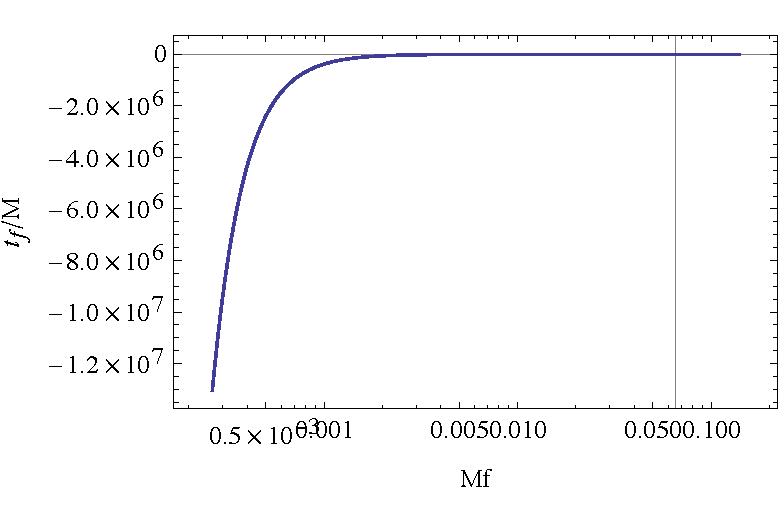
\includegraphics[width=.48\linewidth]{plots/tf.pdf}
  \hspace{0.2cm}
  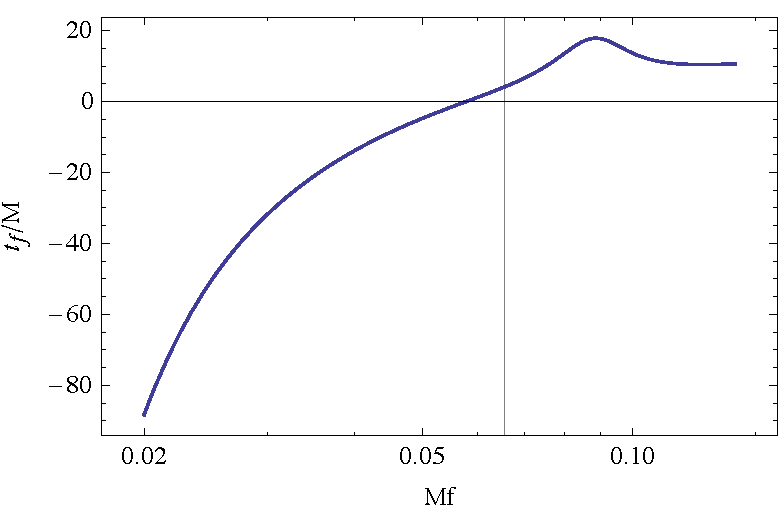
\includegraphics[width=.48\linewidth]{plots/tfzoom.pdf}
  \caption{Time-to-frequency correspondence, as defined directly from the phase of the Fourier-domain signal as in~\eqref{eq:deftf}, in geometric units for an equal-mass, non-spinning system. The right panel shows the merger and ringdown part of the signal in more details. The time axis is such that the time-domain amplitude peaks at $t=0$. The vertical line shows the instantaneous frequency at the peak, and the fact that the curve $t_{f}$ does not pass exactly by the crossing of the two lines reflects the fact that the link between time-domain frequency and Fourier-domain f is not accurate anymore in the merger part of the signal. Note that $t_{f}$ does not go beyond $20M$ after the peak, and is not monotonous.}
  \label{fig:tf}
\end{figure}

Using this notation, we have simply
%
\be\label{eq:local}
	\tilde{s}_{\rm local}(f) = \tilde{h}(f) g(f, \tf) \,.
\ee
%
The interpretation of this approximation is straightforward: the signal is simply multiplied by the response function evaluated at the time $\tf$. Additionally, when delays are present, the frequency-dependence of the response is evaluated directly at $f$. For precessing binary, this corresponds to the approximation used for the PhenomP approximant~\cite{Hannam+13}, as will be discussed in Sec.~\ref{}.

It is worth noting that a shift in time of the time-domain signal will, by construction, be appropriately propagated to~\eqref{eq:local}. If $h'(t) = h(t -  \Delta t)$ [but the modulation and delays are left unchanged (which is relevant for space-based detectors, not for precessing binaries)], $\Psi'(f) = \Psi(f) - 2\pi f \Delta t$, so that
%
\be\label{eq:localshifted}
	\tilde{s}'_{\rm local}(f) = \tilde{h}'(f) g(f, \tf + \Delta t) \,. 
\ee
%
This observation also justifies that the first derivative of the Fourier-domain phase cannot, in general, be considered a small quantity, as it can take arbitrary values for arbitrary shifts in time of the signal. The leading order approximation corresponds to neglecting the curvature in $\Psi(f)$, and yields a result~\eqref{eq:local} where the passage to the Fourier domain is done by simply using a time-to-frequency correspondence~\eqref{eq:deftf}, which motivates the name ``local approximation''.

%%%%%%%%%%%%%%%%%%%%%%%%%%%%%%%%%%%%

\subsection{General Taylor expansion in the Fourier domain}
\label{subsec:TaylorFD}

We now extend our approach beyond the LLP approximation. We will give a formal derivation of the  general formula for the higher-order corrections in~\eqref{eq:FDkernel}, and then specialize it to the special cases of interest.

We will formally Taylor-expand $\tilde{h}(f-f')$ in $f'$ as follows: we write
%
\begin{subequations}
\begin{align}
	\Psi(f-f') &= \Psi(f) + 2\pi f' \tf + \sum\limits_{p\geq 2}^{N} \frac{(-1)^{p}}{p!} {f'}^{p} \frac{\ud^{p} \Psi}{\ud f^{p}} \,, \label{eq:expandPsi}\\
	A(f-f') &= A(f) \sum\limits_{q\geq 0} \frac{(-1)^{q}}{q!} {f'}^{q} \frac{1}{A}\frac{\ud^{q} A}{\ud f^{q}} \,, \label{eq:expandA}\\
	\tilde{g}(f-f', f') &= \sum\limits_{r\geq 0} \frac{(-1)^{r}}{r!} {f'}^{r} \frac{\partial^{r} }{\partial f^{r}}  \tilde{g}(f,f') \label{eq:expandg}
\end{align}
\end{subequations}
%
This expansion will only be usable in practice when we will be able to keep only a few terms in each of these expansions. We therefore limited the expansion in $\Psi$ to a finite order $N$, to keep the formula readable. Notice that we expand $\tilde{g}(f-f',f')$ in $f'$ only in its first argument. We can also interchange the $f$-derivatives of $g$ with its Fourier transform.

If we further expand the exponentials to obtain a pure $f'$-expansion, by applying the derivative rule
\be
	\int \ud f'\, {f'}^{n} \frac{\partial^{m} }{\partial f^{m}}  \tilde{g}(f,f') e^{-2i\pi f' \tf} = \frac{1}{(-2i\pi)^{n}} \left( \frac{\partial^{m} }{\partial f^{m}} \frac{\partial^{n} }{\partial t^{n}} g \right)(f,\tf) \,,
\ee
we arrive at the formal expansion
\begin{align}
	\tilde{s}(f) &= \tilde{h}(f) \sum\limits_{q\geq 0} \sum\limits_{r\geq 0} \sum\limits_{k_{2}\geq 0} \dots \sum\limits_{k_{N}\geq 0} \frac{(-1)^{q}}{q!} \frac{(-1)^{r}}{r!} \prod\limits_{p=2}^{N} \frac{1}{k_{p}!}\left( \frac{(-1)^{p}(-i)}{p!} \frac{\ud^{p}\Psi}{\ud f^{p}}\right)^{k_{p}} \frac{1}{A} \frac{\ud^{q} A}{\ud f ^{q}} \frac{1}{(-2i\pi)^m} \left( \frac{\partial^{r} }{\partial f^{r}} \frac{\partial^{m} }{\partial t^{m}} g \right)(f,\tf) \,,
\end{align}
where $m = p+r+2k_{2}+\dots+N k_{N}$.

This rather cumbersome expression will not be used as such, but is easy to simplify for special cases. For instance, if we expand only the frequency-dependence of $g$ as in~\eqref{eq:expandg}, we obtain
\be\label{eq:taylordelay}
	\tilde{s}(f) = \tilde{h}(f) \sum\limits_{r\geq 0} \frac{1}{(2i\pi)^{r}r!} \left( \frac{\partial^{r} }{\partial f^{r}} \frac{\partial^{r} }{\partial t^{r}} g \right)(f,\tf)
\ee
which interestingly looks like a Taylor expansion of $g$, but with joint derivatives in frequency and time. Similarly, the expansion~\eqref{eq:expandA} gives
\be\label{eq:resultdfA}
	\tilde{s}(f) = \tilde{h}(f) \sum\limits_{q\geq 0} \frac{1}{(2i\pi)^{q}q!} \frac{1}{A} \frac{\ud^{q} A}{\ud f ^{q}}  \left( \frac{\partial^{q} }{\partial t^{q}} g \right)(f,\tf)
\ee

Of particular interest for us will be the case where we keep only the first term in~\eqref{eq:expandPsi}, and expand the resulting exponential, which yields
\be\label{eq:resultdffPsi}
	\tilde{s}(f) = \tilde{h}(f) \sum\limits_{p\geq 0} \frac{1}{p!} \left( \frac{i}{8\pi^{2}}\frac{\ud^{2} \Psi}{\ud f^{2}} \right)^{p} \left( \frac{\partial^{2p} }{\partial t^{2p}} g \right)(f, \tf) \,.
\ee
Indeed, this correction will be the most significant correction beyond leading order in the applications that we will consider in Secs.~\ref{} and~\ref{}, and this particular approximation will turn out to be closely related to the approach of~\cite{Klein+14}.

In the following, it will be convenient to introduce figures of merit of these Taylor-like expansions. Thus we define
\begin{subequations}\label{eq:deffom}
\begin{align}
	\epsilon_{\Psi 2} &\equiv \frac{1}{4\pi^{2}} \left| \frac{\ud^{2} \Psi}{\ud f^{2}} \frac{1}{g} \frac{\partial^{2} g}{\partial t^{2}}(f, \tf) \right| \,, \\
	\epsilon_{A 1} &\equiv \frac{1}{2\pi} \left| \frac{1}{A}\frac{\ud A}{\ud f} \frac{1}{g} \frac{\partial g}{\partial t}(f, \tf) \right| \,, \\
	\epsilon_{A 2} &\equiv \frac{1}{4\pi^{2}} \left| \frac{1}{A}\frac{\ud^{2} A}{\ud f^{2}} \frac{1}{g} \frac{\partial^{2} g}{\partial t^{2}}(f, \tf) \right| \,, \\
	\epsilon_{d} &\equiv \frac{1}{2\pi} \left| \frac{1}{g} \left( \frac{\partial^{r} }{\partial f^{r}} \frac{\partial^{r} }{\partial t^{r}} g \right)(f, \tf) \right| \,.
\end{align}
\end{subequations}

We found in both the LISA case and in the precession case that the third and higher derivatives of both the amplitude and phase are negligible. Note that the figure of merit $\epsilon_{d}$, introduced to represent the effect of the frequency dependence in the convolution kernel~\eqref{eq:FDkernel}, is signal-independent and depends only on $g$.

%%%%%%%%%%%%%%%%%%%%%%%%%%%%%%%%%%%%

\subsection{Signal-dependent timescales and relation to the stationary phase approximation}
\label{subsec:linkSPA}

\begin{figure}
  \centering
  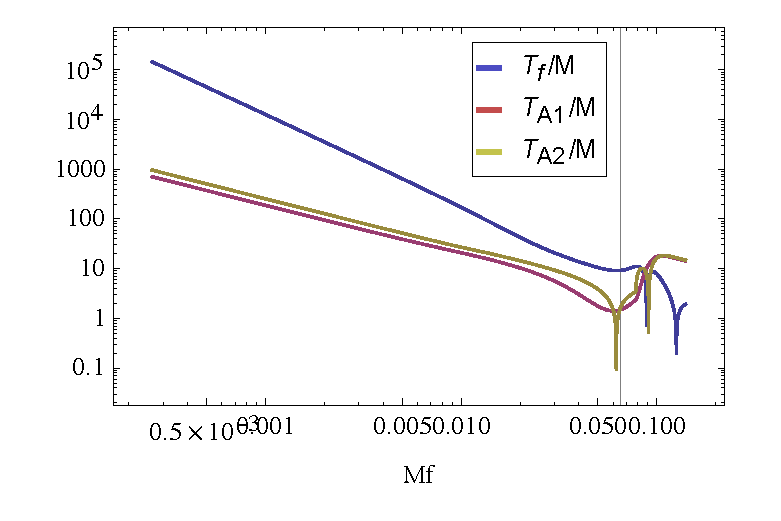
\includegraphics[width=.48\linewidth]{plots/TfTA.pdf}
  \hspace{0.2cm}
  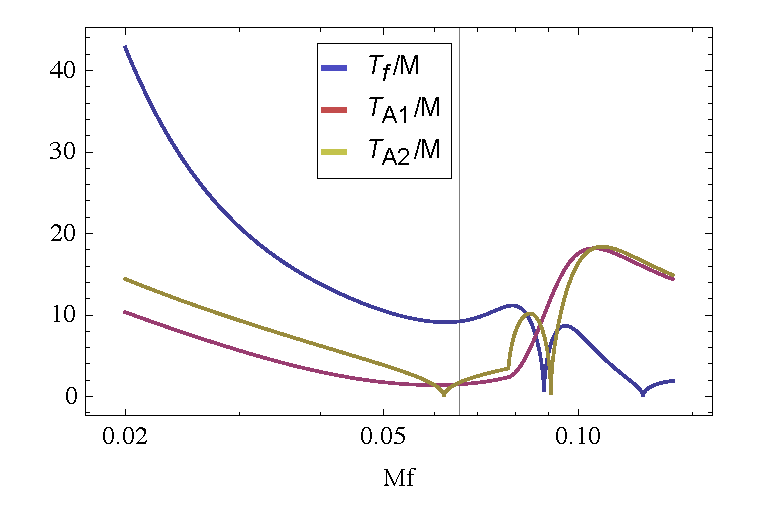
\includegraphics[width=.48\linewidth]{plots/TfTAzoom.pdf}
  \caption{Fourier-domain amplitude and phase timescales, as defined in~\eqref{eq:defTf} and~\eqref{eq:defTA}, in geometric units for an equal-mass, non-spinning system. The right panel shows the merger and ringdown part of the signal in more details, the time-domain frequency at merger being represented by the vertical line. The derivatives from which these timescales are built encounter zero-crossings in the high-frequency range.}
  \label{fig:TfTA}
\end{figure}

Considering~\eqref{eq:eq:resultdffPsi} it is natural to define a new timescale, as a function of frequency, as
\be\label{eq:defTf}
	\Tf^{2} = \frac{1}{4\pi^{2}}\left| \frac{\ud^{2}\Psi}{\ud f^{2}} \right| \,.
\ee
The interpretation of this timescale for the inspiralling part of the signal, when the SPA applies, will be discussed below. Whe can use this notation to rewrite~\eqref{eq:resultdffPsi} as
\begin{align}\label{eq:resultdffPsiTf}
	 \tilde{s}(f) &= \tilde{h}(f) \sum\limits_{p\geq 0} \frac{(-i\epsilon)^{p}}{2^{p}p!} \Tf^{2p} \left( \frac{\partial^{2p} }{\partial t^{2p}} g \right)(f, \tf) \,,
\end{align}
with $\epsilon = -\mathrm{sgn}(\ud^{2}\Psi/\ud f^{2} )$.

The expansion in amplitude corrections~\eqref{eq:resultdfA} also leads to the natural introduction of a set of other timescales related to the successive derivatives of te amplitude. In an analogous manner to the definition~\eqref{eq:defTf} of the timescale $T_{f}$, we can define
\be\label{eq:defTA}
	\left( T_{An} \right)^{n} \equiv \frac{1}{(2 \pi)^{n}} \frac{1}{A(f)} \left| \frac{\ud^{n} A}{\ud f^{n}} \right| \,,
\ee
where we included an absolute value to accomodate the possible sign changes in the right-hand side. In practice, only the first few of these timescales will be relevant.

Of particular interest is the relation between out formal results and the SPA. For non-precessing gravitational wave signals, the SPA is a very good approximation through the inspiralling phase~\cite{Droz+99}. However, it is important to note that the approximation breaks down when reaching the merger-ringdown part of the signal, as the rapidly varying features of the merger break the locality of the time-to-frequency relation~\eqref{eq:deftfSPA}.  

Taking the first derivative of the defining relation~\eqref{eq:deftfSPA} gives
\be
	t_{f} = -\frac{1}{2\pi} \frac{\ud \Psi_{\rm SPA}}{\ud f} \,,
\ee
which means that our generalized definition~\eqref{eq:deftf} for the effective time $t_{f}$ coincides with $t_{f}^{\rm SPA}$ in the inspiral phase of the signal, where the SPA is applicable. Similarly, if we define
\be
	T_{f}^{\rm SPA} \equiv \frac{1}{\sqrt{2\dot{\omega}(t_{f})}} \,,
\ee
we have
\be
	\left(T_{f}^{\rm SPA} \right)^{2} = -\frac{1}{4\pi^{2}}  \frac{\ud^{2} \Psi_{\rm SPA}}{\ud f^{2}} \,,
\ee
where $\ud^{2}\Psi/\ud f^{2} < 0$ in the SPA with our sign conventions. Comparing with~\eqref{eq:defTf} above, we see that our generalized time scale $\Tf$ also reduces to $T_{f}^{\rm SPA}$ when the SPA applies. However, its definition extends to the merger-ringdown part of the signal, and we have to include an absolute value to allow for a possible change of sign of $\ud^{2}\Psi/\ud f^{2}$ in that regime, as shown in Fig.~\ref{fig:TfTA}.

We can now compare our result to the approach of Ref.~\cite{Klein+14}, where the authors extend the SPA in a formalism called the shifted uniform asymptotic expansion (SUA). The derivation includes an expansion of the modulation in Bessel functions, a study of the displacement of the stationary phase point induced by the precession, and a resummation of the result in the form of time derivatives. The main result of~\cite{Klein+14}, their equation~(34), reads exactly like~\eqref{eq:resultdffPsiTf} with the identifications $\tilde{H}_{corr}(f)\rightarrow \tilde{s}(f)/\tilde{h}(f)$ for the transfer function, $T\rightarrow \Tf$ for the radiation-reaction timescale and $e^{-i\delta\phi} \rightarrow F$ for the modulation function (which is restricted in their framework to include only the phase of the modulation, its amplitude being treated jointly with the amplitude of the signal). Thus, we are able to make a direct correspondence between the treatment of~\cite{Klein+14} and our framework, which provides us with a simple and alternative derivation of their result. Namely, the result of~\cite{Klein+14} corresponds to the approximation~\eqref{eq:expandPsi}, where in the Fourier-domain convolution the phase of the signal is expanded to quadratic order and the amplitude is not expanded.

%%%%%%%%%%%%%%%%%%%%%%%%%%%%%%%%%%%%
%%%%%%%%%%%%%%%%%%%%%%%%%%%%%%%%%%%%

\section{Quadratic phase corrections and delays}
\label{sec:quadphasedelay}

%%%%%%%%%%%%%%%%%%%%%%%%%%%%%%%%%%%%

\subsection{Resummation of derivatives for quadratic term in the phase}
\label{subsec:resumquadphase}

In this Section, we focus on the second-derivative corrective term in~\eqref{}. We will restrict to the case of a pure modulation, $d=0$ and $g(f,t) = F(t)$. The authors of~\cite{Klein+14} proposed a resummation scheme. Indeed, the result~\eqref{} looks like a symmetrized Taylor expansion, except for the factors $i^{p}$ and $1/p!$ instead of $1/(2p)!$. After having truncated the sum at some finite $N$, one can write
%
\begin{align}\label{eq:resumquadphase}
	\tilde{s}(f) &\simeq \tilde{h}(f) \sum\limits_{p = 0}^{N} \frac{(-i\epsilon\Tf^{2})^{p}}{2^{p}p!} \partial_{t}^{2p}F(\tf) \nn\\
	&\simeq \tilde{h}(f) \sum\limits_{p= 0}^{N} \sum\limits_{k=0}^{N} a_{N,k}\frac{(k\Tf)^{2p}}{(2p)!}  \partial_{t}^{2p}F(\tf) \nn\\
	&\simeq \tilde{h}(f) \frac{1}{2}\sum\limits_{k=0}^{N} a_{N,k} \left( F(\tf + k\Tf) + F(\tf-k\Tf) \right)\,,
\end{align}
%
where we applied a truncation approximation at the first and last stage. The second equality holds provided that the complex coefficients $a_{N,k}$ are a solution of the $N+1$-dimensional linear system
\be\label{eq:combsystem}
	(-i\epsilon)^{p} (2p-1)!! = \sum\limits_{k=0}^{N} a_{N,k} k^{2p} \quad \text{for } p=0,\dots,N \,.
\ee
The two solutions for the comb coefficients in the two cases $\epsilon = \pm 1$ are simply related by a complex conjugation.

An immediate advantage of this reformulation is its improved numerical stability. For the signal of precessing binaries, although one should expect an ideal scaling $\partial_{t}^{p} F \sim \Omega^{p} F$ with $\Omega$ the precession frequency, it can be extremely hard to control numerical derivatives of $F$ (which in any realistic model will be only provided as sampled at discrete times) well enough to enforce this scaling. Here, however, one simply evaluates the original smooth function $F$ at shifted times.

Note that the choice of the samples $\tf \pm k\Tf$ to approximate the successive derivatives of the expansion by finite differences is by no means unique. In principle, one could have made any ansatz of samples for the series expansion to be matched on. One cannot expect all choices to work equally well when applied to noisy data, and the problems of the numerical size of the coefficients and of the overall numerical stability of the scheme must be investigated numerically.

However, we remark that the transformation~\eqref{eq:resumquadphase} between the two series above has a special structure, and the resulting linear system can be written as a Vandermonde system. Defining the Vandermonde matrix $V(x_{0},\dots,x_{N})$ as $V_{ij} = (x_{j})^{i}$ (with the convention $0^{0} = 1$), setting $x_{j} = j^{2}$, and $b_{p} \equiv (-i\epsilon)^{p}(2p-1)!!$, the linear system~\eqref{eq:combsystem} becomes
\be
	b_{p} = \sum\limits_{k=0}^{N} V_{p,k} a_{N,k} \,.
\ee
Now, since the Vandermonde system solves the Lagrange polynomial interpolation problem, we know that $({}^{t}V^{-1})_{ij}$ is the coefficient of $X^{i}$ in the polynomial $\prod_{k\neq j} (X-x_{k})/(x_{j} - x_{k})$. If we introduce the symmetric polynomials $\sigma$ such that
\be	
	\sigma(m, \{x_{1}, \dots, x_{n}\}) = \sum\limits_{1\leq i_{1}<\dots<i_{m}\leq n} x_{i_{1}}\dots x_{i_{m}} \,,
\ee
we obtain for the inverse of the matrix $V$
\be
	V^{-1}_{ij} = \frac{1}{\prod_{k\neq i} (i^{2} - k^{2})} (-1)^{N-j} \sigma(N-j, \{0,\dots,N^{2}\}\backslash \{i^{2}\}) \,.
\ee
This allows us to write a closed-form expression for the $a_{N,k}$, for every finite order $N$:
\be
	a_{N,k} = \sum\limits_{p=0}^{N} (-i\epsilon)^{p}(2p-1)!! \frac{(-1)^{N-p}}{\prod_{j\neq k} (j^{2}-k^{2})} \sum\limits_{\substack{ 0 \leq i_{1} < \dots < i_{N-p} \leq N \\ i_{1}, \dots, i_{N-p} \neq k}} i_{1}^{2}\dots i_{N-p}^{2}
\ee
The combinatorial explosion of the number of terms in the symmetric polynomials, however, makes this expression impractical to evaluate for $N$ beyond a few dozen. We leave a more complete investigation of the asymptotics and numerical stability of this resummation approach for future work.

%%%%%%%%%%%%%%%%%%%%%%%%%%%%%%%%%%%%

\subsection{Quadratic term in the phase and Fresnel transform}
\label{subsec:fresneltransform}

We can give an alternative interpretation of~\eqref{eq:resultdffPsi} and of Sec.~\ref{subsec:resumquadphase} above by using an integral approach. For simplicity of notation, here we will again keep to the case of precessing binaries, with only a modulation $F$ and no delays, $d=0$. We will reintroduce the delays below in Sec.~\ref{subsec:delays}. To obtain~\eqref{eq:resultdffPsi}, we expanded fully the exponential as a Taylor series. If it is not expanded, however, we have
\be\label{eq:integralquadphase}
	\tilde{s}(f)	\simeq \tilde{h}(f) \int \ud t\, F(t) \int\ud f'\, e^{2i\pi f' (t-\tf)} \exp\left[ 2i\pi^{2} \epsilon{f'}^{2} \Tf^{2} \right] \,,
\ee
where we recall that $\epsilon = -\mathrm{sgn}(\ud ^{2} \Psi/\ud f^{2})$. The integral on $f'$ is a simple complex Gaussian integral, and results in a complex Gaussian integral over time where we recognize a Fresnel transform~\cite{} of the function $F$. We introduce for the Fresnel transform the notation
\be\label{eq:defFresnel}
	\calF_{\tau}[F](t_{0}) \equiv \frac{e^{i\frac{\pi}{4}}}{\sqrt{2\pi} \tau} \int \ud t \, \exp\left[ - \frac{i}{2} \left( \frac{t-t_{0}}{\tau} \right)^{2}\right] F(t) \,,
\ee
together with the additional notation
\be\label{eq:Fresnelsign}
	\calF^{\epsilon}_{\tau}[F](t_{0}) \equiv
\begin{cases}
	 \calF_{\tau}[F](t_{0}) &\text{ if } \epsilon=1 \\
	 \calF_{\tau}[F^{*}](t_{0})^{*} &\text{ if } \epsilon=-1
\end{cases}
\ee
to accomodate for the possible sign change represented by $\epsilon$. The integral~\eqref{eq:integralquadphase} then reads
\be\label{eq:resultFresnel}
	\tilde{s}(f) = \tilde{h}(f) \calF^{\epsilon}_{\Tf}[F](\tf) \,.
\ee

The Fresnel transform is an integral transform that shares some properties with the Fourier transform. It intervenes in particular in the theory of diffraction~\cite{}. Contrarily to the Fourier transform, however, it is localized in the sense that the part of the integral that is centered around $t_{0}$ contributes predominantly, due to the cancelling oscillations far from $t_{0}$. Note also that only the part of the function $F$ that is symmetric about $t_{0}$ contributes to the integral in~\eqref{eq:defFresnel}.

The parameter $\tau$ of the transform plays the role of a focusing parameter, determining how local the transform is. In the limit $\tau\rightarrow 0$, fast oscillations away from the central value $t_{0}$ will cancel out, leading to the integral taking the value $F(t_{0})$. For large values of $\tau$, however, the integral~\eqref{eq:defFresnel} has an extended support. Transposed in terms of the timescale $\Tf$, since we have seen that $\Tf$ can be interpreted as the radiation reaction timescale in the SPA regime, this means that a faster-chirping signal ($\Tf$ small) will have a Fresnel transform that is more focused, whereas a slower-chirping signal ($\Tf$ large) will have a Fresnel transform that is more extended. How much the Fresnel transform is focused in time is to be put in relation with how fast the function $F(t)$ in the integrand is varying. In the case of signals from precessing binaries, the precession timescale evolves as the system gets closer to merger, as will be discussed in details in~\ref{subsec:sizecorrPrec} below. In the case of the response of a LISA-like detectors, the modulation evolves with a timescale of one year, as will be detailed in Sec.\ref{subsec:sizecorrLISA}.

Although it is interesting to be able to relate our results to a known transformation used in signal processing, whether this opens avenues for more efficient computation methods remains to be investigated, for instance by performing a decomposition of the modulation $F$ in chirplets, which have analytically computable Fresnel transforms. Note that in the result~\eqref{eq:resultFresnel}, both the scale $\Tf$ and the central time $\tf$ are functions of the frequency $f$.

As a verification, upon performing a formal Taylor expansion in time of $F(t)$ around $\tf$ in the above integral and integrating term by term the result\footnote{Note that the intermediate integrals produced by such a Taylor expansion are formally divergent. One can regularize them for instance by introducing a small imaginary part in $\tau$ that and sending it to $0$ at the end of the computation.}, one readily recovers our previous result~\eqref{eq:resultdffPsiTf}. Now, the resummation of~\eqref{eq:resumquadphase} can be rephrased as a quadrature rule for computing the Fresnel integral~\eqref{eq:defFresnel}, according to
\be\label{eq:Fresnelstencil}
	\calF_{\tau}^{\epsilon} [F](t_{0}) \simeq \frac{1}{2} \sum\limits_{k=0}^{N} a_{N,k}^{\epsilon} \left( F(t_{0} + k\tau) + F(t_{0} - k\tau) \right)\,,
\ee
with $a_{N,k}^{1} = a_{N,k}$ and $a_{N,k}^{-1} = a_{N,k}^{*}$. Formally, if one allows for polynomial integrands in~\eqref{eq:defFresnel} (which can only be given sense by introducing a regularization), Eq.~\eqref{eq:Fresnelstencil} amounts to the building a quadrature rule for the particular choice of nodes $t_{0} \pm k \tau$, which is exact (with a regularization) if $F$ is a symmetric polynomial of degree $\leq 2N$. Note however that this quadrature rule does not fall into the class of Gaussian quadratures, which provide $N$-point rules that give an exact representation of the integral for polynomials of degree $2N-1$. Due to the complex character of the kernel in~\eqref{eq:defFresnel}, the induced inner product is not positive definite and some key properties are lost, such as the construction of the optimal Gaussian nodes from the zeros of the orthonormalized polynomials. For more details on quadrature rules when applied to integrals with oscillatory kernels, we refer to~\cite{}.

%[TO CORRECT AND REWRITE]
%The rewriting of~\eqref{eq:resultdffPsiTf} by means of an integral transform leads by analogy to another way of formulating the connection to the results of Ref.~\cite{Klein+14}. If we consider the inspiralling phase of a precessing binary, the SPA applies to the signal $h(t) = a(t)e^{-2i\varphi(t)}$. Refering to~\eqref{} above, if we consider as before that $a(t)$ is slowly variable
%\be
%	\tilde{s}(f) \simeq \tilde{h}_{\rm SPA} (f) \simeq a(t_{f}^{\rm SPA}) \exp\left[2i\pi f t_{f}^{\rm SPA}-2i%\varphi(t_{f}^{\rm SPA}) \right]  \int \ud t \, F(t) e^{-i \dot{\omega} (t_{f}^{\rm SPA}) (t-t_{f}^{\rm SPA})^{2}} \,.
%\ee
%We see that, within the context of the SPA, the result~\eqref{} for the quadratic term in the phase, equivalent to the result of~\cite{Klein+14}, can be recovered by a time-domain approach. However, our formalism is somewhat more general, as it does not make use of the SPA for the underlying signal $\tilde{h}(f)$ and can in principle be used for the merger-ringdown part of the signal as well.

%%%%%%%%%%%%%%%%%%%%%%%%%%%%%%%%%%%%

\subsection{Treatment of the delays}
\label{subsec:delays}

In the case of a LISA-type detector response, the presence of the delay $d(t)$ is responsible for the frequency-dependence of the kernel $g$ introduced in~\eqref{eq:defg}. We will show below in Sec.~\ref{} that the higher-order correction in the delay can become non-negligible at high frequencies, as measured by the magnitude of the first correction in~\eqref{eq:taylordelay}. This is especially true for the orbital delay related to the motion of the whole detector constellation around the Sun, due to the large baseline for this delay.

Here we give an alternative treatment of the delays which is an alternative to the mere Taylor expansion of~\eqref{eq:taylordelay}. It is useful to look first at the case where one neglects the signal-related amplitude and phase corrections as given in~\eqref{eq:resultdfA} and~\eqref{eq:resultdffPsiTf}, but keeps the frequency-dependence in the convolution kernel in~\eqref{eq:defg}. The response then depends on the signal only by the time-to-frequency correspondence and reads
\begin{equation}
	\tilde{s}(f) = \tilde{h}(f) \int \ud t \, F(t) e^{-2i\pi f d(t)} \int \ud f' \, e^{2i\pi f' (t+d(t) - t_{f})} \,,
\end{equation}
where we recall that we defined $t_{f} \equiv -1/(2\pi)\ud \Psi/\ud f$. This motivates the introduction of the delayed time function $t_{d}:t \mapsto t+d(t)$, and of the reciprocal function $t_{d}^{-1}$, and of a modified time-to-frequency correspondence $\tfd = t_{d}^{-1}(\tf)$, defined implicitly by
\be
	\left. (t + d(t) - t_{f})\right|_{t=t_{f}^{d}} = 0 \,.
\ee
The above integral can then be formally computed as
\begin{align}\label{eq:delaycorrleading}
	\tilde{s}(f) &= \tilde{h}(f) \int \ud t \, F(t) e^{-2i\pi f d(t)} \delta(t + d(t) - t_{f}) \nn \\
	&= \tilde{h}(f) F(t_{f}^{d}) \frac{e^{-2i\pi f d(t_{f}^{d})}}{1+\dot{d}(t_{f}^{d})}
\end{align}

For the standard LISA configuration, we have for the orbital delays the scaling $d_{O}\sim R/c \sim 500s$, for the constellation delays the scaling $d_{c}\sim L/c \sim 17s$ (with an additional dependence on angular factors). Since the motion of the constellation is periodic with a period of one year and $\Omega_{0} = 2.10^{-7}\mathrm{rad}.s^{-1}$, we have $\dot{d}_{O} \sim \Omega_{0} R/c \sim 10^{-4}$ and $\dot{d}_{c} \sim \Omega_{0} L/c \sim 3.10^{-6}$. The smallness of the dimensionless quantity $\dot{d} \ll 1$ (and of its subsequent derivatives) will allow us to treat it perturbatively with a very good approximation, and shows also that the function $t_{d}$ is univalued and that there is no ambiguity in defining its reciprocal $t_{d}^{-1}$.

By treating $\dot{d}$ as a perturbation and keeping only first-order terms, we obtain for the delayed time reciprocal function
\begin{align}
	t_{d}^{-1}(t) &\simeq t-d(t) (1-\dot{d}(t)) \,,\nn\\
	d(t_{f}^{d}) &\simeq d(t_{f}) ( 1 - \dot{d}(t_{f})) \,.
\end{align}
Now, the most relevant correction in~\eqref{eq:delaycorrleading} comes from the phase factor at high frequencies, where the factors $2\pi f d_{O}$ and $2\pi f d_{c}$ give a magnification by a factor of, respectively, $3.10^{3}$ and $10^{2}$ at $1\Hz$. Ignoring the other corrections, we thus arrive at the approximate form
\be
	\tilde{s}(f) \simeq \tilde{h}(f) F(t_{f})\exp\left[ -2i\pi f d(t_{f}) (1-\dot{d}(t_{f})) \right] \,.
\ee
Notice that this leading-order correction in the treatment of the delays affects purely the phase of the signal.

Next, we consider the case where the quadratic phase correction is kept as well, as in Sec.~\ref{subsec:fresneltransform}. Keeping as before only the first-order terms in $\dot{d}$ (and neglecting its higher derivatives), we can write
\begin{align}
	\tilde{s}(f) &\simeq \tilde{h}(f) \int \ud t \, F(t) e^{-2i\pi f d(t)} \int \ud f' \, \exp\left[ 2i\pi \epsilon \Tf^{2} f'^{2} + 2i\pi f' (t+d(t) - \tf) \right] \nn\\
	&\simeq \tilde{h}(f) \frac{e^{i\epsilon\frac{\pi}{4}}}{\sqrt{2\pi}\Tf} \int \ud \tau \, \frac{F(\tau - d(\tau))}{1+\dot{d}(\tau)} e^{-2i\pi f d(\tau)(1-\dot{d}(\tau))}\exp\left[ -\frac{i\epsilon}{2} \frac{(\tau - \tf)^{2}}{\Tf^{2}} \right] \,,
\end{align}
where we used a change of variable $\tau = t_{d}(t)$. We see that the result can again be expressed as a Fresnel transform.

When considering amplitude corrections as well, as in~\eqref{}, additional powers of $f'$ can be translated as time derivatives with respect to the variable $\tau$ after performing the change of variables. Thus, we obtain our most general result for an exact treatment of the quadratic term in the phase and for an improved treatment of the delays as:
\be
	\tilde{s}(f) = \tilde{h}(f) \sum\limits_{k=0}^{+\infty} \frac{1}{(2i\pi)^{k} k!} \frac{1}{A} \frac{\ud^{k}A}{\ud f^{k}}  \calF^{\epsilon}_{\Tf} \left[ \frac{\ud^{k}}{\ud \tau^{k}} \left( \frac{F(\tau - d(\tau))}{1+\dot{d}(\tau)} e^{-2i\pi f d(\tau)(1-\dot{d}(\tau))} \right) \right] (\tf) \,.
\ee
Each term in this series (in practice, only the first few will be relevant) can in turn be approximated by using the stencil formula~\eqref{eq:Fresnelstencil}.

%%%%%%%%%%%%%%%%%%%%%%%%%%%%%%%%%%%%
%%%%%%%%%%%%%%%%%%%%%%%%%%%%%%%%%%%%

\section{Application to the response of LISA-type detectors}
\label{sec:LISA}

%%%%%%%%%%%%%%%%%%%%%%%%%%%%%%%%%%%%

\subsection{The response model and TDI observables}
\label{subsec:modelLISA}

In this Section, we expand Sec.~\ref{subsec:} and detail more the model that we use for the response of a LISA-like detector, together with the assumptions used and their limitations.

As argued in~\cite{Krolak+04}, since we focus on the gravitational-wave contribution to the basic observable, we can use a simplified model for the response, ignoring corrections that are crucial from the point of view of noise cancellations. Our aim is indeed to assess the accuracy of a direct Fourier-domain treatment of the response, thus focusing on the separation of timescales in the problem, keeping in mind that corrections can be added later without affecting the conclusions of the present analysis.

The frequency-shift response for a single link~\eqref{eq:yslr} was derived in Ref.~\cite{EW75} (see also~\cite{} for a more modern version). Several assumptions enter the result as written in~\eqref{eq:yslr}: (i) effects of the order $v/c$ are neglected, including for instance the special relativistic Doppler effect created by the relative speeds of the spacecrafts on their orbits (ii) the propagation is assumed to take place in a flat spacetime, perturbed only by the gravitational wave; thus the gravitational redshift as well as the deflection of light created by the gravitational potential of the Sun is ignored (iii) all geometric factors are evaluated at a single time, whereas one should consider the beam as propagating from the position of the first spacecraft at the time of emission to the position of the second scapecraft at the time of reception, leading to a pointing-ahead effect.

Additionally, we limit ourselves to a rigid model for the detector, namely we assume that the constellation remains in an equilateral configuration with fixed armlengths $L=5.10^{6}\mathrm{km}$. This simplified orbits neglect (iv) the effect of excentricity of the individual Keplerian orbits, which introduces corrections at the level $e^{2}$ (v) the effect of gravitational perturbations coming from other celestial bodies, such as the Earth, the quadrupole of the Sun, and the other planets. 

Although all the effects (i)-(v) are neglected here, keeping track of these corrections is crucial for the purpose of noise cancellations, and led to the development of new generations of TDI observables~\cite{}.

We now turn to the transposition of~\eqref{eq:yslr} to the Fourier-domain. We will choose to write the response directly in terms of spin-weighted spherical modes $h_{\ell m}$, whose Fourier transforms are assumed to have a smooth amplitude and phase. Since the orbital delay due to the orbit around the Sun is common to all $y_{slr}$ observables, we will decompose the response in the orbital delay and the constellation-centered response as
\begin{subequations}
\begin{align}
	h^{\rm TT}_{O} (t) &\equiv h^{\rm TT}(t-\hat{k}\cdot p_{O}) \,, \label{eq:dfresponseO} \\
	y_{slr} &= \frac{1}{2} \frac{1}{1 - \hat{k}\cdot n_{l}} n_{l}\cdot \left[ h_{O}^{\rm TT}(t - \hat{k}\cdot p^{L}_{s}) - h_{O}^{\rm TT}(t - \hat{k}\cdot p^{L}_{r}) \right] \cdot n_{l}\,, \label{eq:dfresponsec}
\end{align}
\end{subequations}
where we introduced the positions of the spacecrafts relative to the center of the constellation, $p^{L}_{A} \equiv p_{A} - p_{O}$.

When using the rigid approximation for the constellation, a particular simplification occurs when writing the transfer function at leading order in the delays. First, we define the matrices $P^{+},P^{\times}$ such that
\be
	h^{\rm TT} = h_{+}P_{+} + h_{\times}P_{\times} \,,
\ee
in the sense of matrices. The spin-weighted spherical harmonics factors in~\eqref{eq:hpcfrommodes} are mere constants of time, so we can also define a geometric projection factor $P_{slr}^{\ell m}$ for each individual mode. Under the assumption that we can neglect the negative frequencies for the modes $m>0$ and the positive frequencies for $m<0$ (which is also used for precessing waveforms), we have for $f>0$ and $m>0$
%\begin{subequations}
\begin{align}
	P_{slr}^{\ell m} &= \frac{1}{4} \frac{1}{1-\hat{k}\cdot n_{l}} {}_{-2}Y_{\ell m} n_{l}\cdot \left( P_{+} - i P_{\times} \right) \cdot n_{l} \text{ for } m>0 \,,
\end{align}
%\end{subequations}
the transfer function for~\eqref{eq:dfresponsec} reads in the local approximation
\be
	\calT_{slr}^{\ell m} = \frac{i \pi f L}{2} \sinc \left[ \pi f L\left(1-\hat{k}\cdot n_{l} \right) \right] \exp\left[ \pi f \left( L + \hat{k}\cdot \left( p_{1}^{L} + p_{2}^{L} \right) \right) \right] {}_{-2}Y_{\ell m} n_{l}\cdot \left( P_{+} - i P_{\times} \right) \cdot n_{l} \text{ for } m>0 \,,
\ee
where we used the fact that, in our rigid approximation for the trajectory of the constellation, $p^{L}_{r} - p^{L}_{s} =  L n_{l}$.

Note that, if the corrections~\eqref{} are included for the constellation delays, this transfer function will not have this simple form anymore as $\dot{d}$ will have a different velocity-dependent expression for the sending and receiving spacecrafts.

%%%%%%%%%%%%%%%%%%%%%%%%%%%%%%%%%%%%

\subsection{Estimates for the magnitude of higher-order corrections}
\label{subsec:sizecorrLISA}

Due to the smallness of $\Omega/2\pi \simeq 3.1\times10^{-8}\mathrm{Hz} \ll f$ over all the frequency band we consider, one can expect that . In this Section we try to quantify to which extent. 

The magnitude of the first terms in a Taylor expansion in $f_{0}$ is (taking $10^{-5}\mathrm{Hz}$ as a reference starting frequency):
%
\begin{widetext}
\begin{subequations}
\begin{align}
	\delta_{A1} &\equiv \left| \frac{1}{A_{N}}\frac{\ud A_{N}}{\ud f} f_0 \right| \simeq 3\times10^{-3} \left(\frac{f}{10^{-5}\Hz}\right)^{-1} \,,\\
	\delta_{\Psi 2} &\equiv \left| \frac{1}{2} f_0^{2}\frac{\ud^{2} \Psi_{N}}{\ud f^{2}} \right| \simeq 5 \left( \frac{m}{10^{6}\Msol} \right)^{-5/3} \left( \frac{\nu}{1/4} \right)^{-1} \left( \frac{f}{10^{-5}\Hz} \right)^{-11/3} \,, \\
	\delta_{\Psi 3} &\equiv \left| \frac{1}{6} f_0^{3}\frac{\ud^{3} \Psi_{N}}{\ud f^{3}} \right| \simeq 2\times 10^{-2} \left( \frac{m}{10^{6}\Msol} \right)^{-5/3} \left( \frac{\nu}{1/4} \right)^{-1} \left( \frac{f}{10^{-5}\Hz} \right)^{-14/3} \,.
\end{align}
\end{subequations}
\end{widetext}
%
The approximation degrades for lower starting frequencies, and, at a fixed frequency, when the total mass decreases and/or the mass ratio increases. However, if we consider only merging binaries, that is to say binaries of which the merger is seen during the observation period of the mission, we have a lower limit for the starting frequency which can be larger than the detector's lowest frequency in band.

From the Newtonian estimate~\eqref{}, the starting frequency is then
%
\be
	f_{\rm start} = 10^{-5}\mathrm{Hz} \left( \frac{m}{8.5\times10^{6}\Msol} \right)^{-5/8} \left( \frac{\nu}{1/4} \right)^{-3/8} \left( \frac{\Delta t}{5 \mathrm{yr}} \right)^{-3/8} \,.
\ee
%
So we see that the ``worst'' total mass is $8.5\times10^6\Msol (\nu/(1/4))^{3/5}$, for 5 years of observation and $f_{\rm low} = 10^{-5}\mathrm{Hz}$ for the entry in band, which are conservative values; for higher masses, part of the signal is cut because it is out-of-band, while for lower masses, the signal is cut because of the limited time of observation before merger, and we have the scaling
%
\be
	|\delta^{2}\Psi |_{f_\mathrm{start}} \propto m^{5/8}\nu^{3/8}\Delta t^{11/8} \,,
\ee
%
which shows that the effect of the truncation of the signal for a finite observation time wins: the approximation becomes better for lower mass and higher mass ratios systems. The worse point in the parameter space should be, for these Newtonian estimates, at equal mass and $m=8.5\times 10^{6} \Msol$, with $|\delta^{2}\Psi |_{\mathrm{worst}} \simeq 0.15$.

\begin{figure}
  \centering
  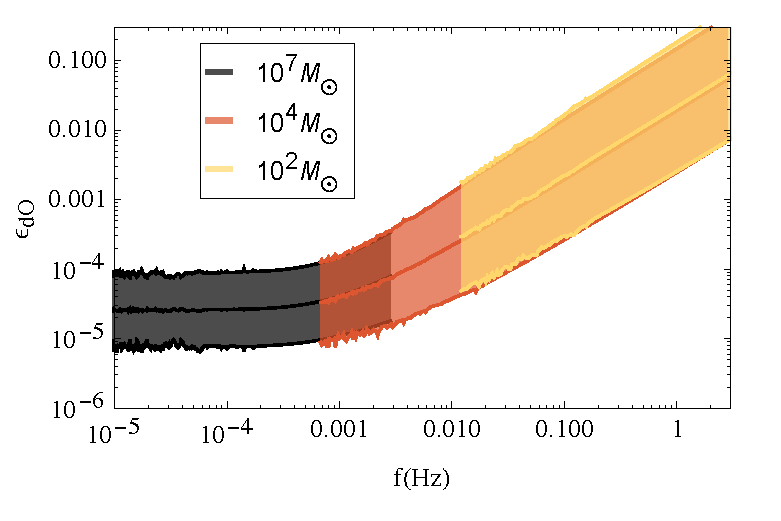
\includegraphics[width=.48\linewidth]{plots/LISAfomdO.pdf}
  \hspace{0.2cm}
  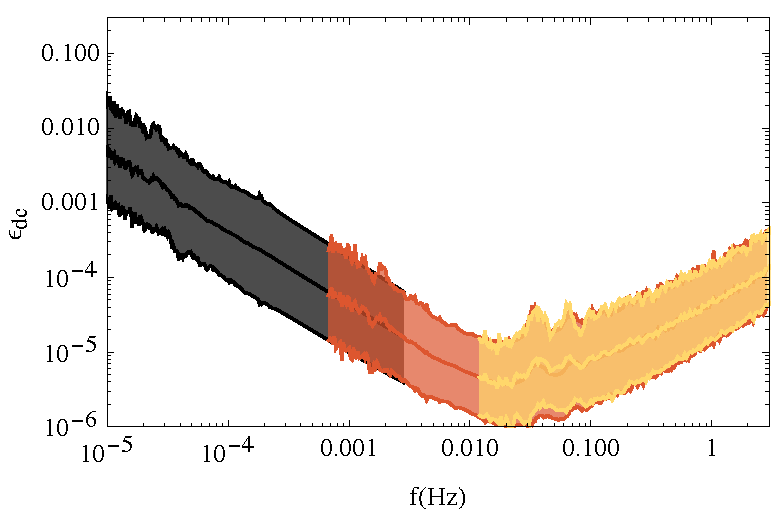
\includegraphics[width=.48\linewidth]{plots/LISAfomdc.pdf}
  %
  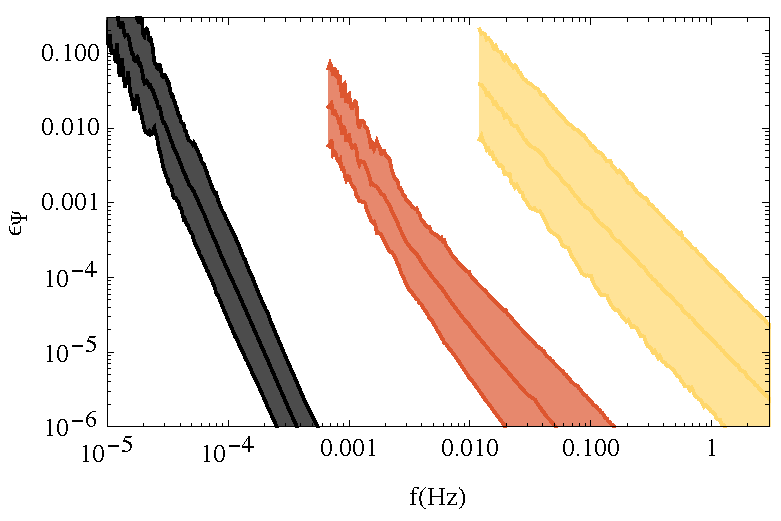
\includegraphics[width=.48\linewidth]{plots/LISAfomPsi2.pdf}
  \hspace{0.2cm}
  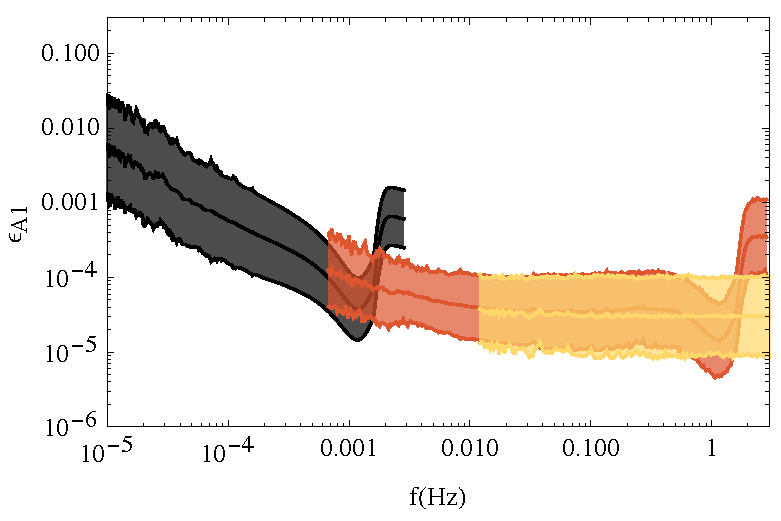
\includegraphics[width=.48\linewidth]{plots/LISAfomA1.pdf}
  \caption{Figures of merit of the approximation as defined in~\eqref{eq:deffom}, for an equal-mass, non-spinning system and for total masses of $10^{7} \Msol$, $10^{4} \Msol$ and $10^{2} \Msol$. The upper left panel corresponds to the orbital delay part of the response~\eqref{eq:dfresponseO}, and the upper right panel corresponds to the LISA-centered response~\eqref{eq:dfresponsec}. The central line and interval are the mean and $1\sigma$ standard deviation of the logarithm of $\epsilon$ over 400 random values for the position in the sky, inclination and polarization.}
  \label{fig:fomLISA}
\end{figure}

Fig.~\ref{fig:fomLISA} shows the magnitude of the figures of merit $\epsilon$ for different total masses, for the orbital delay, for the rest of the response, for the quadratic-in-phase term and for the first derivative of the amplitude. Since individual signals can show significant variation depending on the angular parameters, we show the average over the sky position, inclination and polarization, and $\pm \sigma$ standard deviation.

%%%%%%%%%%%%%%%%%%%%%%%%%%%%%%%%%%%%

\subsection{Error control for the Fourier-domain response}
\label{subsec:errorsLISA}

\begin{figure}
  \centering
  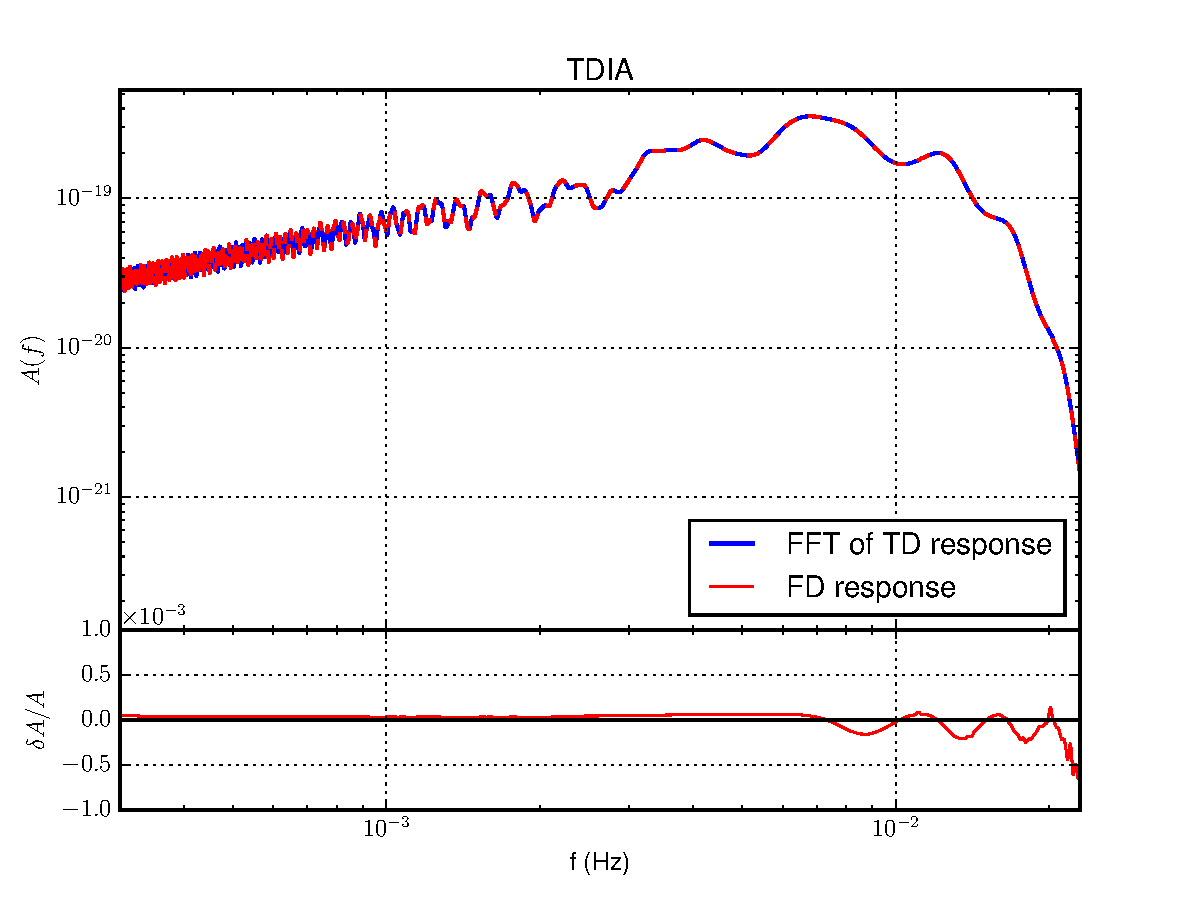
\includegraphics[width=.48\linewidth]{plots/tdifdAamp.pdf}
  \hspace{0.2cm}
  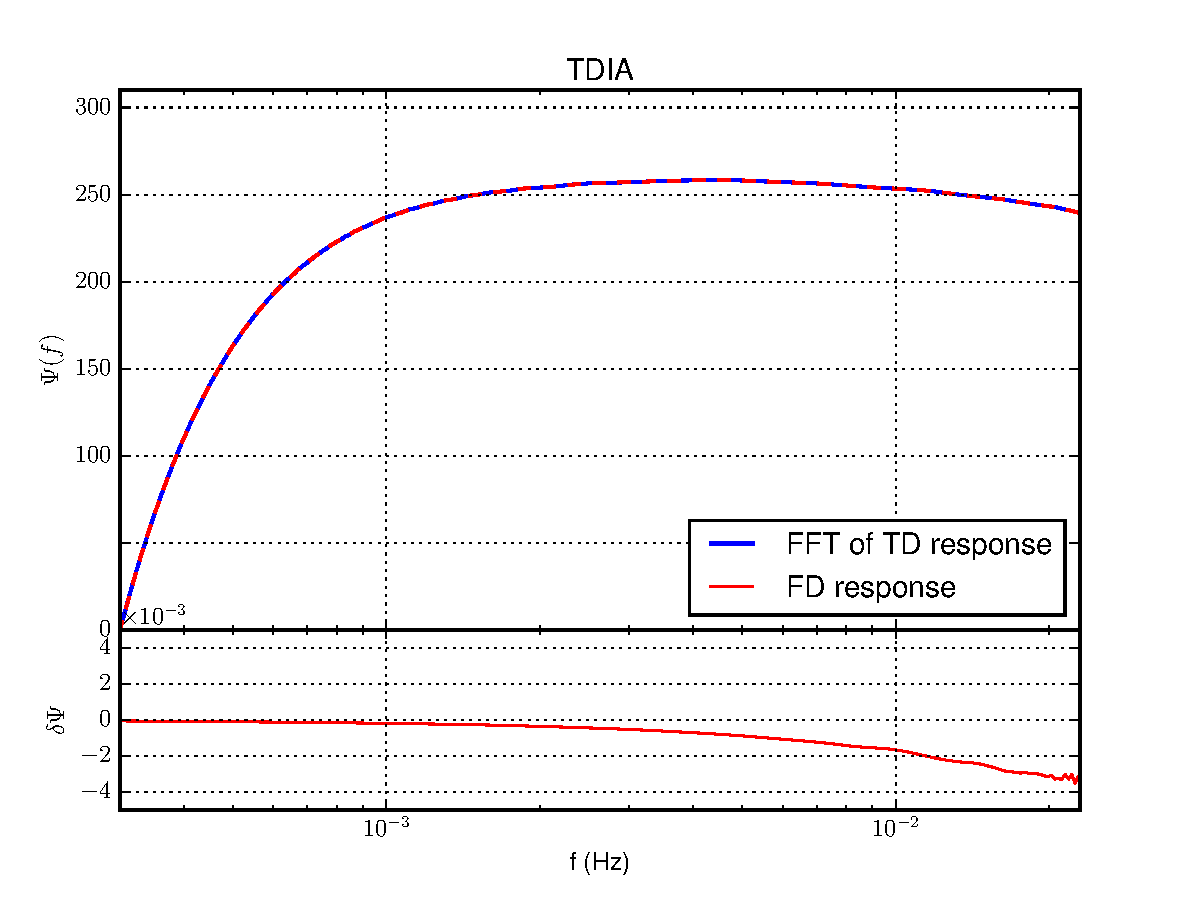
\includegraphics[width=.48\linewidth]{plots/tdifdAphase.pdf}
  \caption{Fourier-domain amplitude and phase timescales, as defined in~\eqref{eq:defTf} and~\eqref{eq:defTA}, in geometric units for an equal-mass, non-spinning system. The right panel shows the merger and ringdown part of the signal in more details, the time-domain frequency at merger being represented by the vertical line. The derivatives from which these timescales are built encounter zero-crossings in the high-frequency range.}
  \label{fig:tdifdA}
\end{figure}

Fig.~\ref{fig:tdifdA} shows the amplitude and phase errors in the Fourier-domain local response when compared to the FFT of the time-domain response~\eqref{eq:yslr}.

%%%%%%%%%%%%%%%%%%%%%%%%%%%%%%%%%%%%
%%%%%%%%%%%%%%%%%%%%%%%%%%%%%%%%%%%%

\section{Application to waveforms from precessing binaries}
\label{sec:Precession}

%%%%%%%%%%%%%%%%%%%%%%%%%%%%%%%%%%%%

\subsection{Simplified model of precessing IMR waveform}
\label{subsec:precmodel}

[explain inertial frame/precessing frame]
[explain Gatech formula for post-merger precession]

Here we will only consider the inertial-frame modes induced by the precessing-frame dominant 22 mode.

[introduce phenomP]
[explain model with smoothing for the angles with its two versions]
[qualify how bad the model is with respect to full NR]

In the following, since our purpose here is not to provide a full-fledged model for precessing signals in the Fourier domain, we will not explore the full parameter space and we will limit our analysis to a simplified toy model for precession. Namely, we will approximate the Euler angles during the inspiral phase by using the PN expressions used in PhenomP~\cite{Hannam+13}, and we will adopt two alternatives asymptotic behaviours post-merger. In the first one (thereafter Case I), we simply send smoothly all three Euler angles to constants. In the second one (Case II), we send the opening angle of the precession cone $\beta$ to a constant, but we reproduce the behaviour describe letting the frame rotate around the direction of the final total angular momentum $\hat{\bm{J}}_{\rm final}$ with an angular velocity of $\Omega_{\rm frame} = \omega_{220} - \omega_{210}$. Fig.~\ref{fig:prectoymodel} shows the Euler angles evolution for Cases I and II.

\begin{figure}
  \centering
  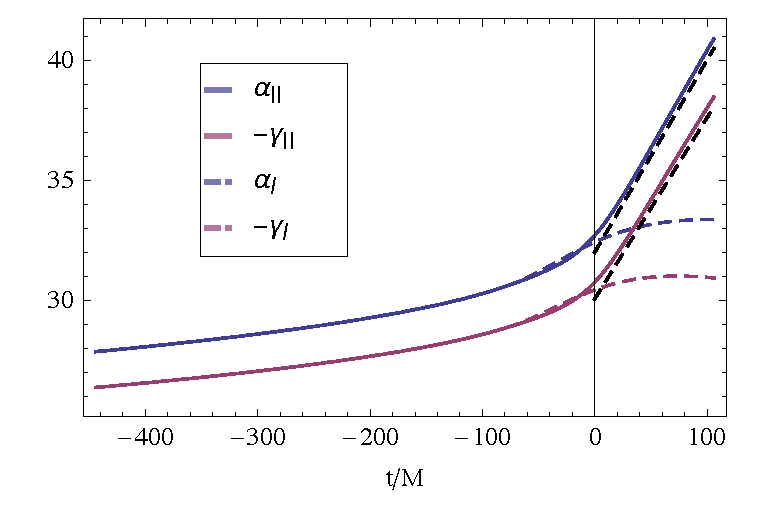
\includegraphics[width=.48\linewidth]{plots/prectoymodelalphagamma.pdf}
  \hspace{0.2cm}
  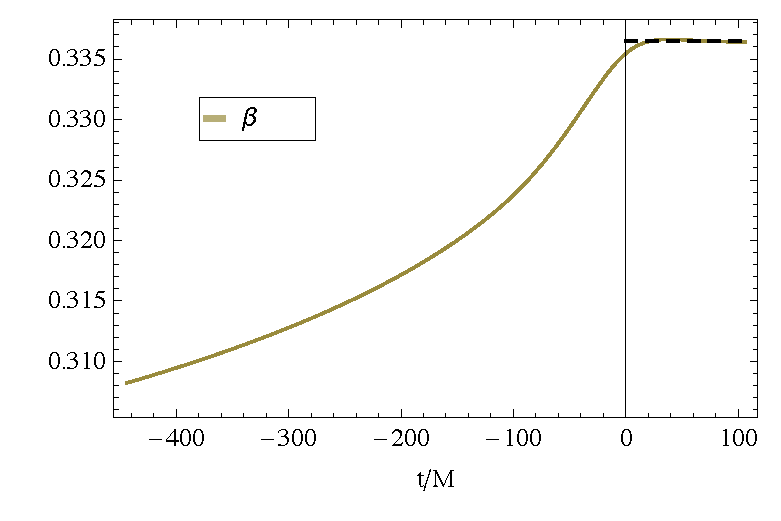
\includegraphics[width=.48\linewidth]{plots/prectoymodelbeta.pdf}
  \caption{Evolution of Euler angles $(\alpha, \beta, \gamma)$ for our two toy models. Dashed lines represent Case I and solid lines Case II. The vertical line indicates the time of merger. Dashed black lines indicate the enforced asymptotic behaviour: frame rotation with angular velocity $\omega_{220} -\omega_{210}$ in Case II, and asymptotically constant $\beta$.}
  \label{fig:prectoymodel}
\end{figure}

These simplifications comes with obvious limitations. Notably, they produce modulation functions $F(t)$ that are very smooth by construction. However, these two toy models will allow us to explore the separation of timescales in the merger-ringdown part of the signal, and to highlight how the perturbative analysis can be challenged by the rapid rotation of the radiation frame after merger, even in this idealized model.

In the absence of delays, we have a simple modulation of the signal by a function $F(t)$, as given in~\eqref{eq:defmodulationprec} above. The convolution with a frequency-dependent kernel~\eqref{eq:FDkernel} becomes a simple convolution in the Fourier-domain,
\be\label{eq:convolution}
	\tilde{s} (f) = \int \ud f' \, \tilde{h}(f-f') \tilde{F} (f') \,.
\ee

It will be convenient to use the notation
\be\label{eq:defFlmlmp}
	F_{\ell m, \ell m'} \equiv D^{\ell *}_{m'm} (\alpha,\beta,\gamma)
\ee
which represents the modulation function corresponding to the contribution of each precessing-frame mode $h^{P}_{\ell m}$ mode to the inertial-frame mode $h^{I}_{\ell m'}$ (see Eq.~\eqref{eq:wignerrot}). One can also define Fourier-domain tranfer functions for each mode contribution, according to
\be\label{eq:defTlmlmp}
	\mathrm{FT} \left[F_{\ell m, \ell m'} h \right] (f) \equiv \calT_{\ell m, \ell m'} (f) \tilde{h}(f) \,,
\ee
where $\mathrm{FT}$ stands sfor the Fourier transform. Fig.~\ref{fig:prectransfer} gives the amplitude and phase of the transfer functions $\calT_{22, 2 m'}$ for the two cases I and II. As expected, the difference between the two toy models for the post-merger frame precession is localized to the high frequency range. One can see a clear hierarchy in the amplitude of the inertial-frame modes generated by the precessing-frame 22 mode. This hierarchy come from the Wigner geometric factors and is dependent on the opening angle of the precession cone, or second Euler angle $\beta$, which in turn is dependent on the magnitude of the misaligned spins in the system. Case II shows stronger amplitude features in the merger and ringdown.

\begin{figure}
  \centering
  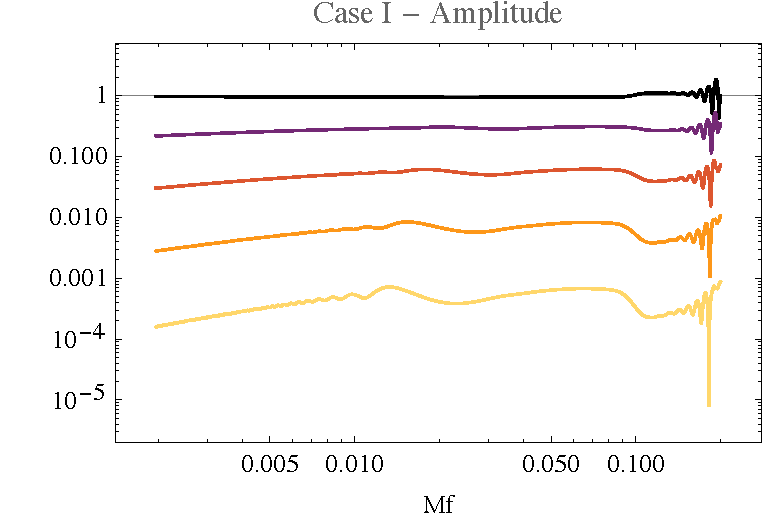
\includegraphics[width=.48\linewidth]{plots/prectransferAcaseI.pdf}
  \hspace{0.2cm}
  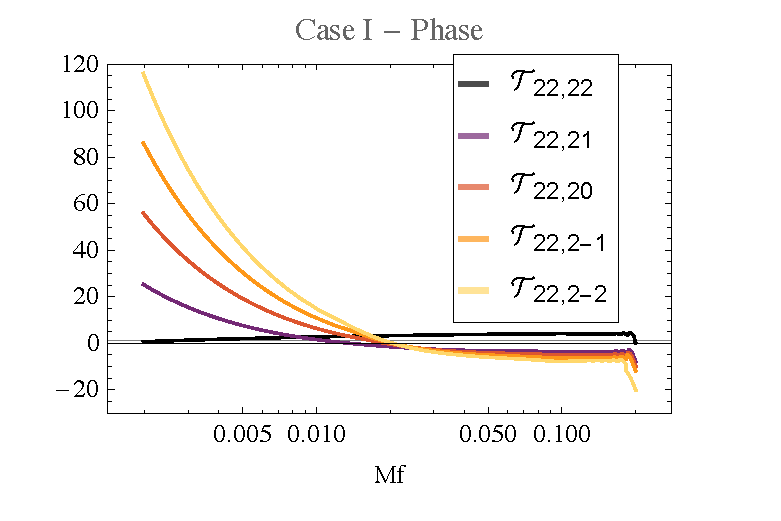
\includegraphics[width=.48\linewidth]{plots/prectransferPsicaseI.pdf}
  %
  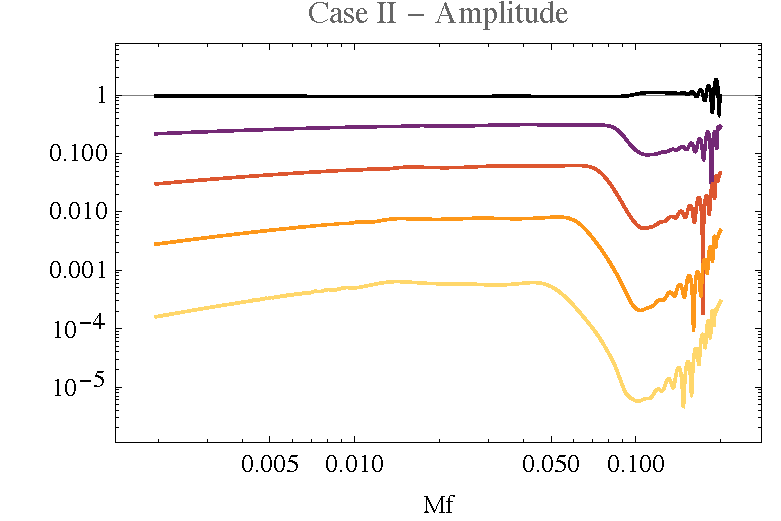
\includegraphics[width=.48\linewidth]{plots/prectransferAcaseII.pdf}
  \hspace{0.2cm}
  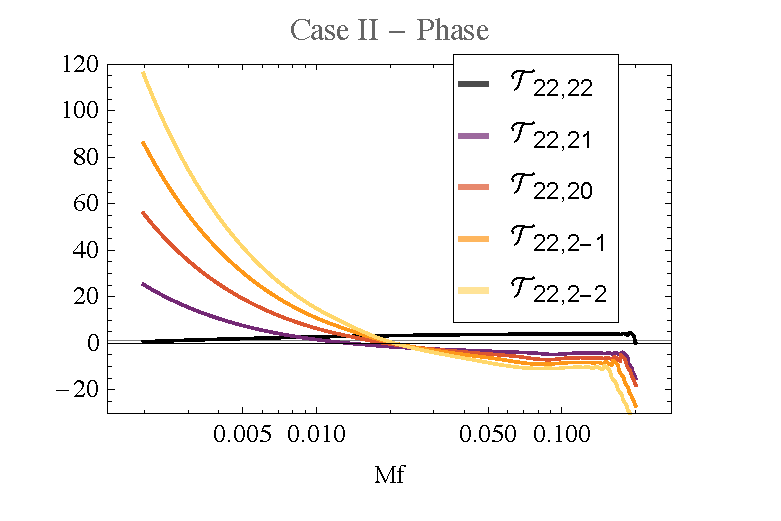
\includegraphics[width=.48\linewidth]{plots/prectransferPsicaseII.pdf}  
  \caption{Amplitude and phase of the Fourier-domain transfer fonctions $\calT_{22,2m'}$ as defined in~\eqref{eq:defTlmlmp} for individual mode contributions. The left panels show the amplitude and the right panels the phase.}
  \label{fig:prectransfer}
\end{figure}

%%%%%%%%%%%%%%%%%%%%%%%%%%%%%%%%%%%%

\subsection{Estimates for the magnitude of higher-order corrections}
\label{subsec:sizecorrPrec}

We investigate now the post-Newtonian order counting of the expansion~\eqref{eq:resultdffPsiTf} during the inspiralling phase of a precessing binary, with modulation $F$ as in~\eqref{}. Using the notation $\calO(n) = \calO(c^{-n})$, we have for quasi-cirular inspirals that $\dot{\omega} = \calO(5)$, corresponding to the radiation reaction effect at the 2.5PN order. The mode mixing will be induced by the rotation of the orbital angular momentum $\bm{L}$ around the total angular momentum $\bm{J}$, with the angular velocity for this precession $\bm{\Omega} = \calO(2)$. The relevant scaling for the terms in the series~\eqref{eq:resultdffPsiTf}, for the inspiral phase where the SPA applies, is therefore
\be
	\Tf^{2p} \partial_{t}^{2p} F = \calO(-1) \,,
\ee
meaning that the expansion becomes {\it less} well behaved for {\it lower} frequencies. The presence of a $1/p!$ gives a formal sense to the expansion if the successive derivatives of $F(t)$ are appropriately bounded, but one may have to keep a large number of terms in the sum. The approximation that consists in taking the first term in the series, the LLP approximation~\eqref{} which was in particular used for the PhenomP~\cite{} waveform model, gets {\it worse} the further away from merger the signal is. [This does not seem to have been clearly stated before, to check]. We investigate further in Sec.~\ref{} the validity of the treatment of precession used for PhenomP.

Notice that, for the amplitude derivatives in~\eqref{eq:expandA} and the higher order derivatives of the phase in~\eqref{eq:expandPsi}, the same PN scaling arguments give however the opposite, more usual behaviour that the terms beyond the first one appear as corrections becoming less and less important at lower frequencies. For instance, within the SPA we obtain
\begin{subequations}
\begin{align}
	\frac{\ud^{3} \Psi}{\ud f^{3}} \frac{1}{F} \partial_{t}^{3} F &= \calO(6) \,, \\
	\frac{1}{A}\frac{\ud A}{\ud f} \frac{1}{F} \partial_{t} F &= \calO(2) \,.
\end{align}
\end{subequations}

\begin{figure}
  \centering
  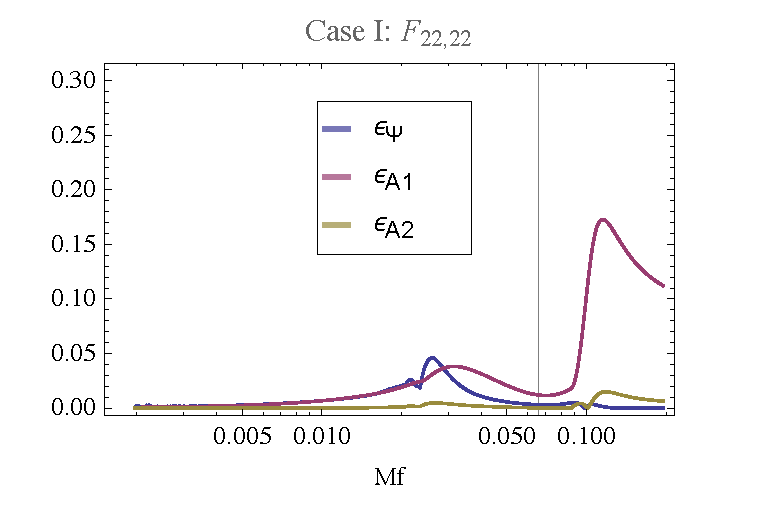
\includegraphics[width=.48\linewidth]{plots/precfom22caseI.pdf}
  \hspace{0.2cm}
  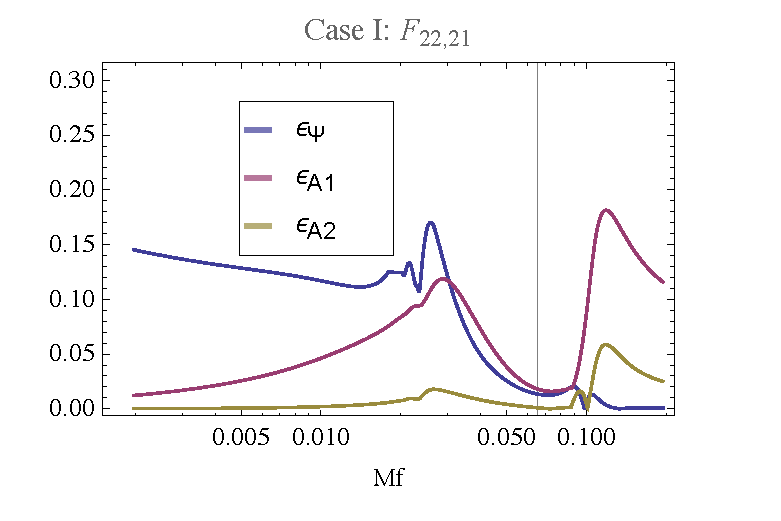
\includegraphics[width=.48\linewidth]{plots/precfom21caseI.pdf}
  %
  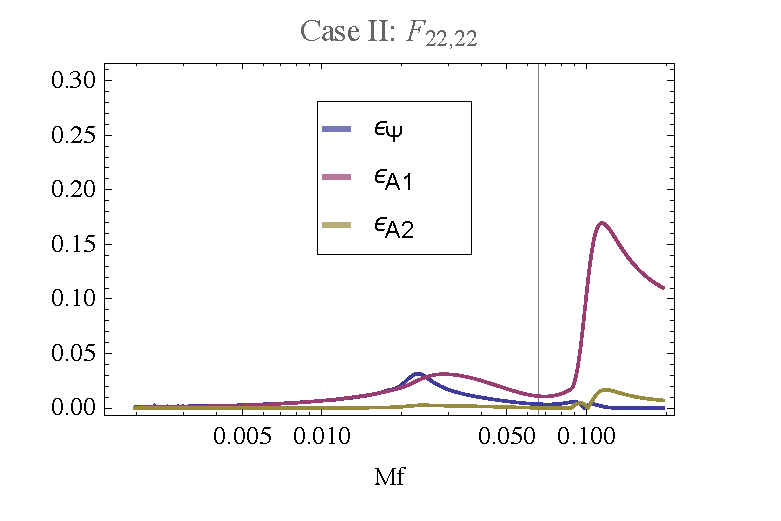
\includegraphics[width=.48\linewidth]{plots/precfom22caseII.pdf}
  \hspace{0.2cm}
  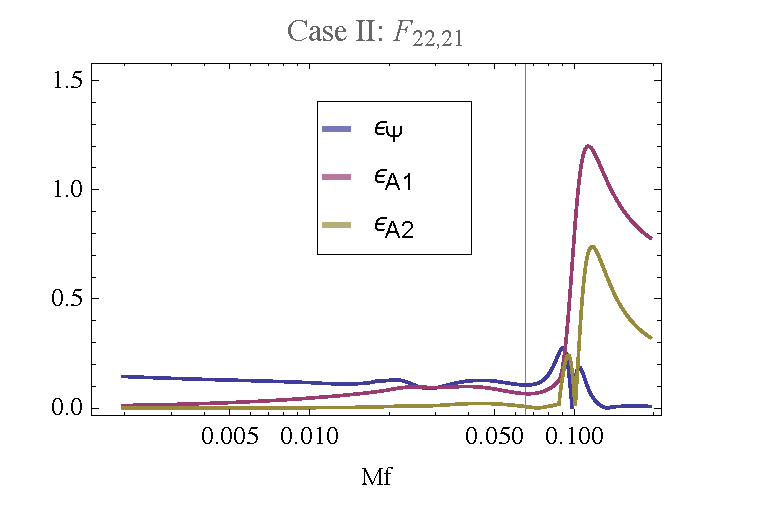
\includegraphics[width=.48\linewidth]{plots/precfom21caseII.pdf}
  \caption{Figures of merit of the approximation as defined in~\eqref{eq:deffom} for the precession modulations. The precessing-frame waveform is taken to be the $22$ mode of an equal-mass, non-spinning system. The two upper panels show the case where the frame rotation is freezed at merger (Case I), while the two lower panels show the case where it rotates after merger (Case II) (see Sec.~\ref{subsec:precmodel} for their definitions). The left panels show the figures of merit for $F_{22, 22}$, and the right panels for $F_{22, 21}$. The vertical line represents the frequency at merger. The amplitude corrections become non-negligible after merger, and become large enough to challenge a perturbative treatment in Case II for $F_{22,21}$ (notice the change of scale for the lower right panel).}
  \label{fig:TfTA}
\end{figure}

%%%%%%%%%%%%%%%%%%%%%%%%%%%%%%%%%%%%

\subsection{Direct convolution approach for the merger-ringdown phase}
\label{subsec:directconvolution}

As will be shown by Fig.~\ref{} below, although including higher-order amplitude corrections does capture some effects near merger, it is not sufficiently accurate and seems to be too sensitive to the details of the evolution of the modulation $F(t)$ in the merger region. Motivated by this shortcoming of the Taylor-like expansion approach, here we investigate an alternative way of handling the merger-ringdown part of the signal.

Thanks to the separation of timescales between the precessional timescale and the orbital timescale, for suffciently high frequencies the convolution~\eqref{eq:convolution} will have a support that will be entirely comprised in the high-frequency part of the signal $\tilde{h}(f)$, which is rather featureless and slowly varying as a function of $f$. Taking advantage of this smoothness, we will adopt a trigonometric polynomial representation for $\tilde{h}(f)$. For frequencies high enough that the support of the convolution~\eqref{eq:convolution} does not extend beyond the range covered by this trigonometric representation, we will be able to write the result directly as a Discrete Fourier Transform (DFT) with a limited number of samples.

We consider the high-frequency part of the signal above some frequency $f_{0}$, up to some maximal frequency $f_{\rm max}$ where the Fourier-domain amplitude of the signal has decayed to a negligible level. In our example of the equal-mass, non-spinning waveform, we take $[Mf_{0}, Mf_{\rm max}] = [0.05, 0.16]$. First, we eliminate a constant and a linear term in the phase by choosing another frequency central to the high-frequency range we want to represent, which we take to be $Mf_{p} = 0.1$. We can think of $f_{p}$ as representing roughly the frequency at merger, and of the associated time $t_{p}\equiv \tf(f_{p})$ as an estimate of the time of merger. Note that the method should only be weakly sensitive to the precise choice of $f_{p}$ and $t_{p}$.

Additionaly, we taper the amplitude to arrive at a flat amplitude at $f_{0}$, at the price of introducing a deviation from the amplitude of the original signal. We localize this deviation to $f\leq f_{1}$, with $Mf_{1} = 0.06$ in our example, and in general the trigonometric representation will be accurate to the original signal only for $f\geq f_{1}$. This tapering is built in practice as the discrete integral of a cosine window function. To ensure good continuity properties, we perform an artificial symmetrization to a fictitious range $f\in [f_{0} - (f_{\rm max} - f_{0}), f_{0}]$, by imposing symmetric amplitudes and phases about $f_{0}$. Defining $\Delta f \equiv 2 (f_{\rm max} - f_{0})$, we write 
\be\label{eq:defhsym}
	\tilde{h}_{\rm sym}(f) = 
	\begin{cases} 
		\exp\left[- i \left( \Psi(f_{0}) - 2i\pi (f-f_{0}) t_{p} \right) \right] \tilde{h}(f) \,,  &\text{ for } f \in [f_{0}, f_{0} + \Delta f /2] \\
	\tilde{h}_{\rm sym}(2 f_{0} - f)^{*} \,,  &\text{ for } f \in [f_{0} - \Delta f/2, f_{0}]
	\end{cases}
\ee

Next, we build a a trigonometric polynomial representation of $\tilde{h}_{\rm sym }$. This construction is intimately related to the DFT, but we recall it for completeness. For a periodic function $f(x)$ defined on $x\in [x_{0}, x_{0} + \Delta x]$, and represented by $N$ samples $x_{j} = \ov{x} + j \Delta x/N$ (with $N$ chosen to satisfy the Nyquist criterion), we can build a trigonometric interpolant $P(x)$ as
\be
	P(x) = \sum\limits_{k=-M}^{+M} c_{k} e^{2i\pi k \frac{x-x_{0}}{\Delta x}}
\ee
that will satisfy the system $P(x_{j}) = f(x_{j})$ for $j=0,\dots, N-1$. Here we set $M=N/2$ (assuming N is even). The coefficients $c_{k}$ are related to the coefficients of the inverse DFT of the series for $f$. If we set $\omega \equiv e^{2i\pi/N}$ and define
\be
	y_{k} = \frac{1}{N} \sum\limits_{j=0}^{N-1} f(x_{j}) \omega^{jk} \,,
\ee
which is the expression of the inverse DFT in our sign convention~\eqref{}, the coefficients $c_{k}$ are given by
\begin{align}\label{eq:ckyk}
	c_{k} &= y_{k} \text{ for } k=0,\dots, M-1 \,, \nn\\
	c_{k} &= y_{k+N} \text{ for } k=-M+1,\dots, -1 \,, \nn\\
	c_{M} &= c_{-M} = \frac{y_{M}}{2} \,,
\end{align}
where the condition $c_{M} = c_{-M}$ is an arbitrary condition enforced to match the number of degrees of freedom. Fig~\ref{fig:convolsymmetrized} shows both the original high-frequency part of the signal and its reconstruction as a trigonometric polynomial.

\begin{figure}
  \centering
  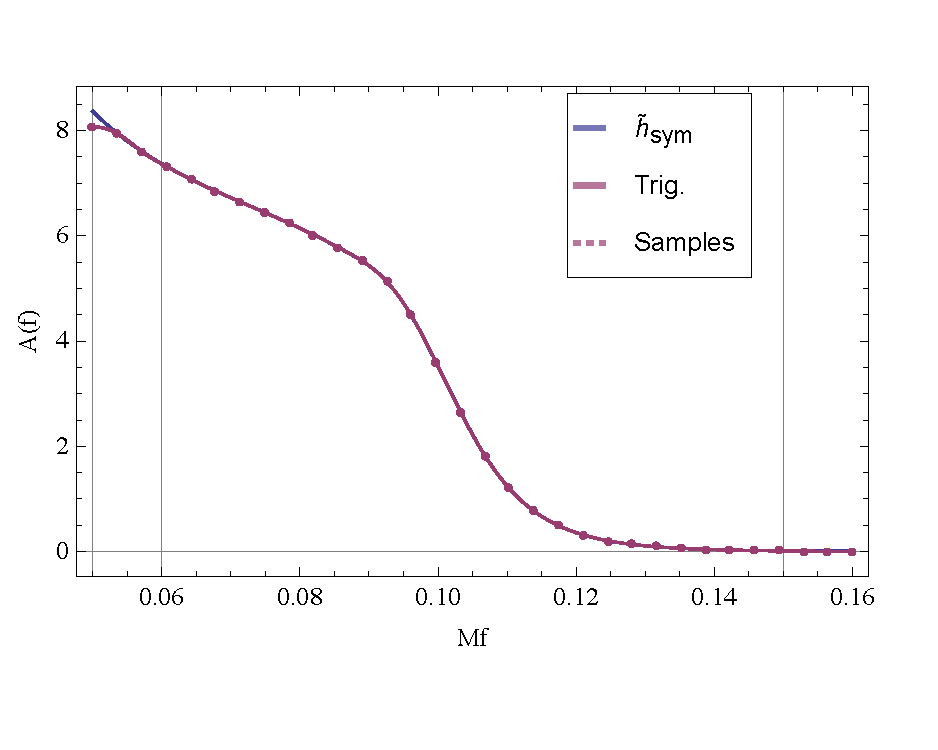
\includegraphics[width=.48\linewidth]{plots/trigamp.pdf}
  \hspace{0.2cm}
  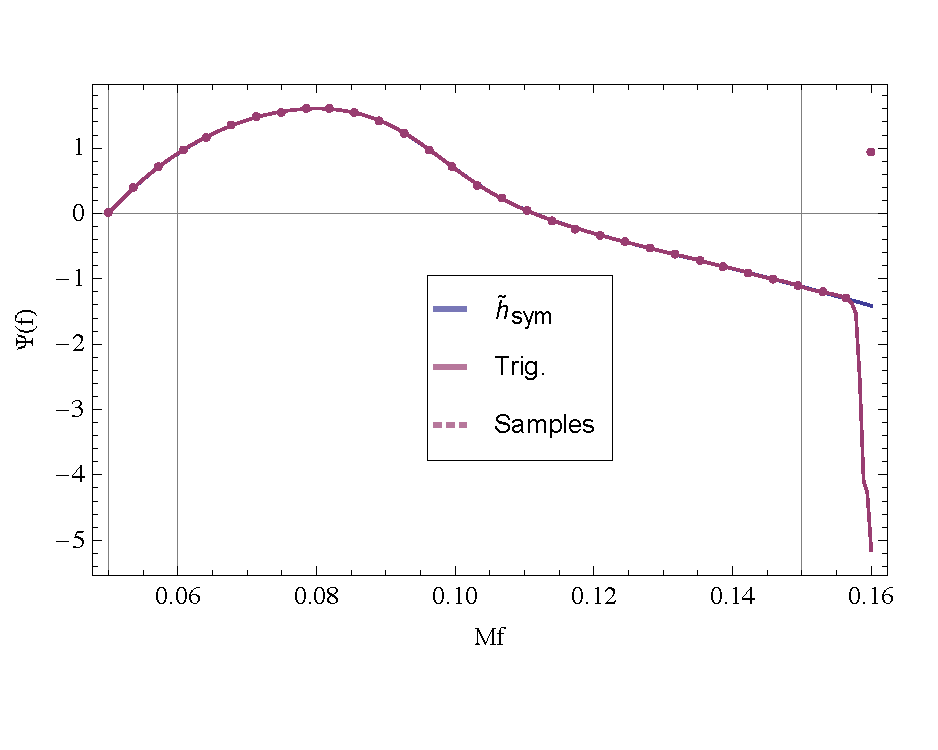
\includegraphics[width=.48\linewidth]{plots/trigphase.pdf}
  \caption{Amplitude (left panel) and phase (right panel) of the high-frequency part of $\tilde{h}_{\rm sym}$, compared to its trigonometric polynomial representation.}
  \label{fig:trig}
\end{figure}

Now, assuming that we wish to compute~\eqref{eq:convolution} for a frequency $f$ such that the extent of the convolution does not extend beyond $[f_{1}, f_{\rm max}]$, we can approximate
\be\label{eq:hsymtrigo}
	\tilde{h}_{\rm sym } (f) \simeq \sum\limits_{k=-M}^{+M} (-1)^{k} c_{k} e^{2i\pi k \frac{f-f_{0}}{\Delta f}} \,,
\ee
where the factor $(-1)^{k}$ comes from the fact that $f_{0}$ is here at the center of the interval. The coefficients $c_{k}$ are built following the rules~\eqref{eq:ckyk} from the inverse DFT coefficients
\be\label{eq:ykDFT}
	y_{k} = \frac{1}{N} \sum\limits_{j=0}^{N-1} \tilde{h}_{\rm sym}\left( f_{0} + \frac{2j - N}{N} \Delta f \right) \omega^{jk} \,.
\ee
When inserting this representation~\eqref{eq:defhsym} and~\eqref{eq:hsymtrigo} into~\eqref{eq:convolution}, we obtain
\be\label{eq:resultdirectconvol}
	\tilde{s}(f) = e^{-i \Psi(f_{0})} e^{2i\pi (f-f_{0}) t_{p}} \sum\limits_{k=-M}^{+M} (-1)^{k} c_{k} e^{2i\pi k \frac{f-f_{0}}{\Delta f}} F(t_{p} + k\delta t) \,, 
\ee
where we defined the time sampling $\delta t \equiv 1/\Delta f$. We see that we are left with a DFT-like expression to compute from $N+1$ time samples of the modulation function $F$, centered around $t_{p}$.

In terms of performance, the implementation of~\eqref{eq:ykDFT} and~\eqref{eq:resultdirectconvol} above is expected to have a very reasonable cost. We obtained results with a good accuracy, as shown in Fig.~\ref{fig:convolsymmetrized}, by including $M=32$ samples ($N=64$ samples in total for the artificially symmetrized signal). The calculation described here is done only once for a given waveform and modulation function. The number of samples is of the same order of magnitude as the number of (logarithmically-spaced) frequency samples used to represent the Fourier-domain waveform with its amplitude and phase in the first place, thus the cost is comparable to the Taylor-like approach presented in Sec.~\ref{sec:quadphasedelay}. 

%%%%%%%%%%%%%%%%%%%%%%%%%%%%%%%%%%%%

\subsection{Error control for the Fourier-domain modulation}
\label{subsec:errorsPrec}

\begin{figure}
  \centering
  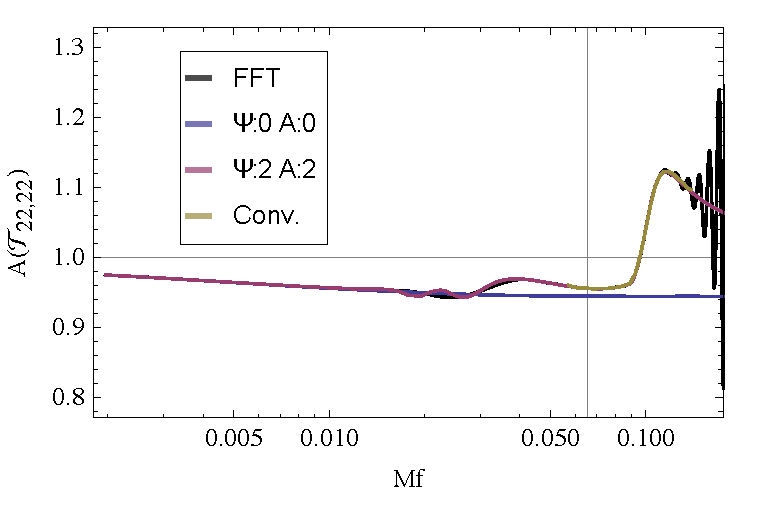
\includegraphics[width=.48\linewidth]{plots/precerrorA22caseI.pdf}
  \hspace{0.2cm}
  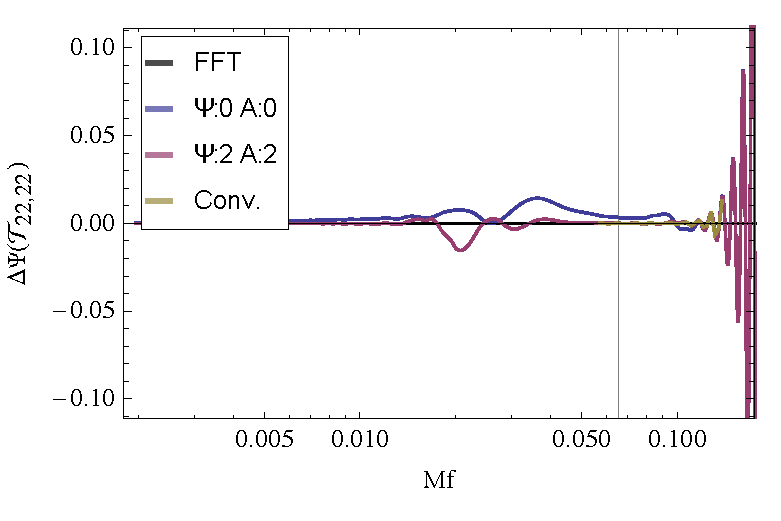
\includegraphics[width=.48\linewidth]{plots/precerrorPsi22caseI.pdf}
  %
  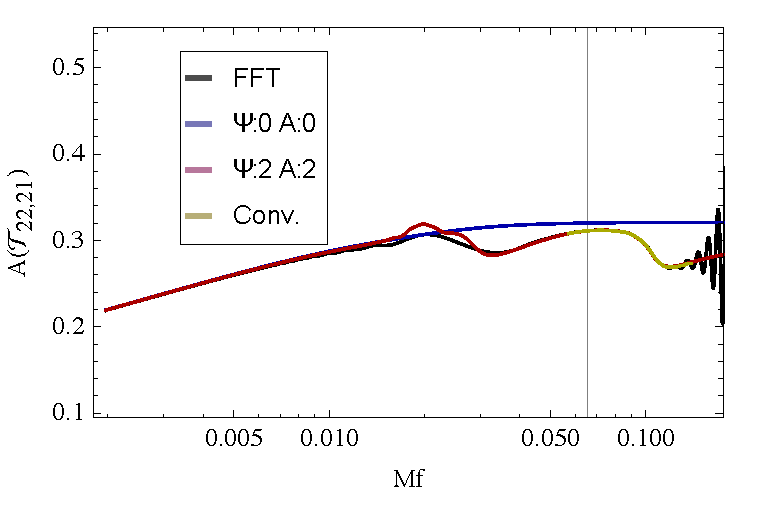
\includegraphics[width=.48\linewidth]{plots/precerrorA21caseI.pdf}
  \hspace{0.2cm}
  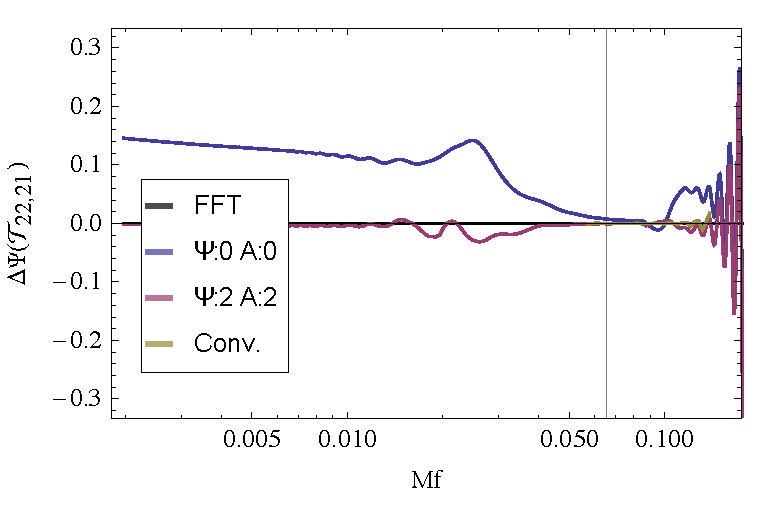
\includegraphics[width=.48\linewidth]{plots/precerrorPsi21caseI.pdf}  
  \caption{Errors in the Fourier-domain transfer fonctions $\calT_{22,22}$ and $\calT_{22,21}$ as defined in~\eqref{eq:defTlmlmp}, for Case I and for various approximations. The black curve is the exact result provided by the FFT. The blue curve gives the leading-order, local approximation. The red curve includes quadratic corrections in phase and in amplitude. The yellow curve shows the result of the direct conolution approach of Sec.~\ref{subsec:directconvolution}. The left panels show the amplitude and the right panels the phase difference with the FFT. Note that the vertical scales are not uniform.}
  \label{fig:precerrorcaseI}
\end{figure}

\begin{figure}
  \centering
  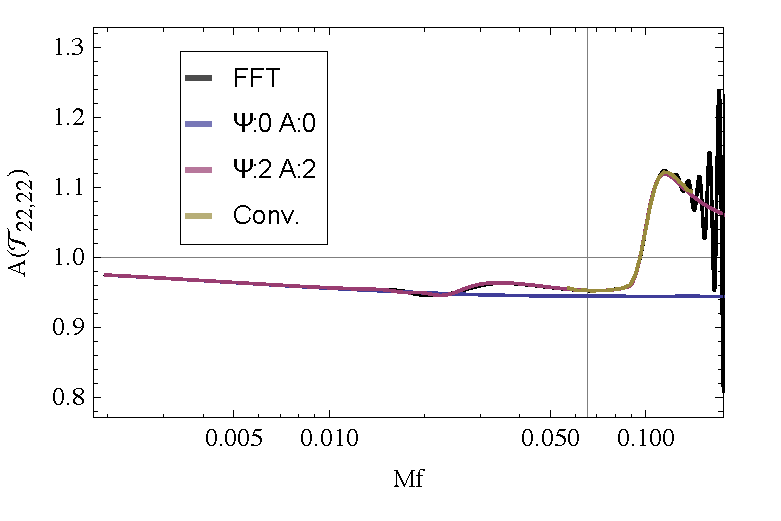
\includegraphics[width=.48\linewidth]{plots/precerrorA22caseII.pdf}
  \hspace{0.2cm}
  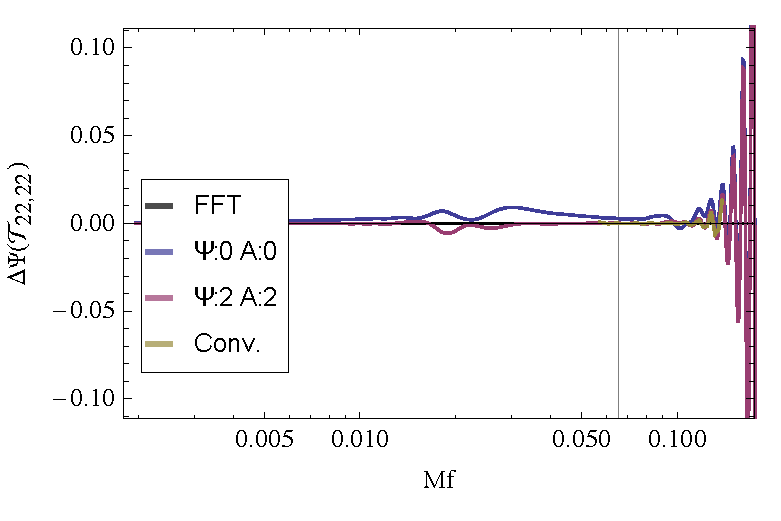
\includegraphics[width=.48\linewidth]{plots/precerrorPsi22caseII.pdf}
  %
  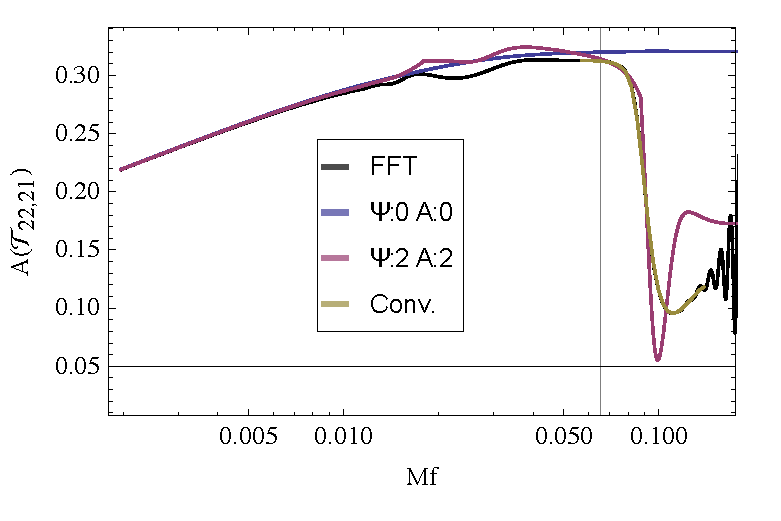
\includegraphics[width=.48\linewidth]{plots/precerrorA21caseII.pdf}
  \hspace{0.2cm}
  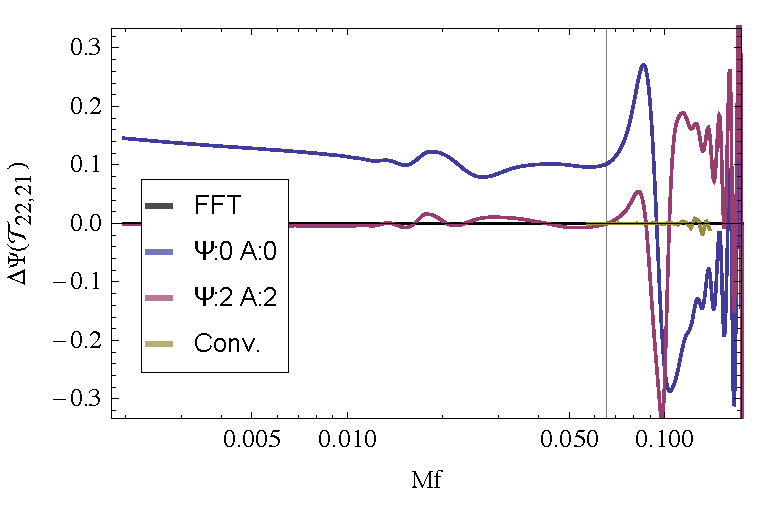
\includegraphics[width=.48\linewidth]{plots/precerrorPsi21caseII.pdf}  
  \caption{Errors in the Fourier-domain transfer fonctions $\calT_{22,22}$ and $\calT_{22,21}$. Conventions are the same as in Fig.~\ref{fig:precerrorcaseI} but for Case II, with a more rapid post-merger frame precession. Note that the vertical scales are not uniform.}
  \label{fig:precerrorcaseII}
\end{figure}

Figs.~\ref{fig:precerrorcaseI} and~\ref{fig:precerrorcaseII} show the amplitude and the phase error of the various reconstructions of the Fourier-domain transfer functions $\calT_{22,22}$ and $\calT_{22,21}$. Alongside with the exact result provided by the FFT of the time-domain precession modulation, we show the result obtained with the leading-order approximation (the local approximation) and with. We also show the result for the direct convolution approach presented in Sec.~\ref{subsec:directconvolution}.

\begin{figure}
  \centering
  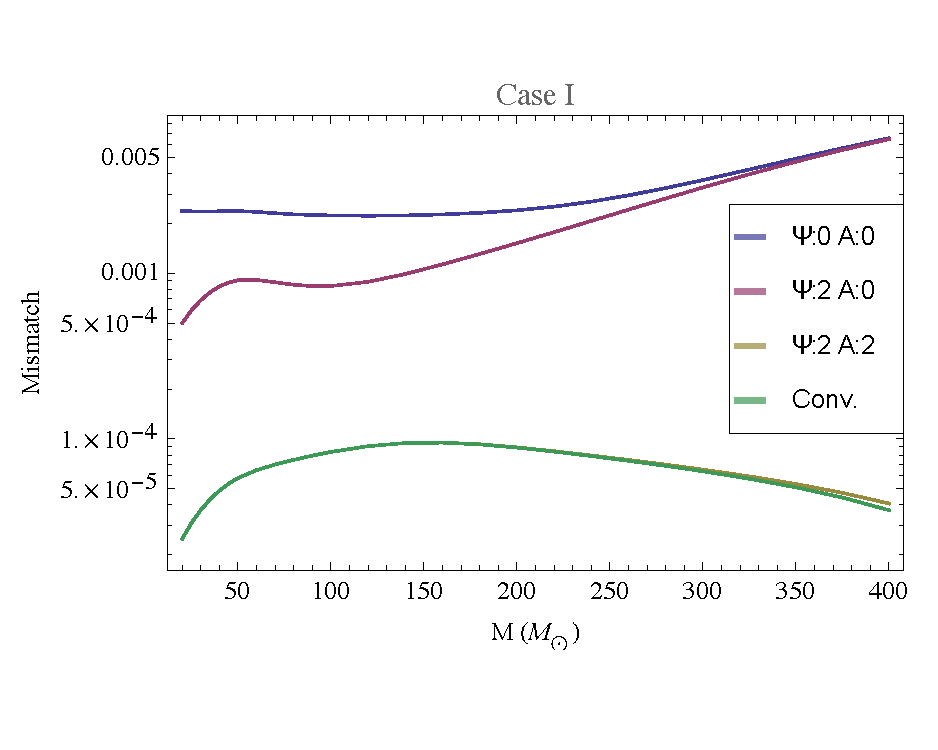
\includegraphics[width=.48\linewidth]{plots/precmmsimple.pdf}
  \hspace{0.2cm}
  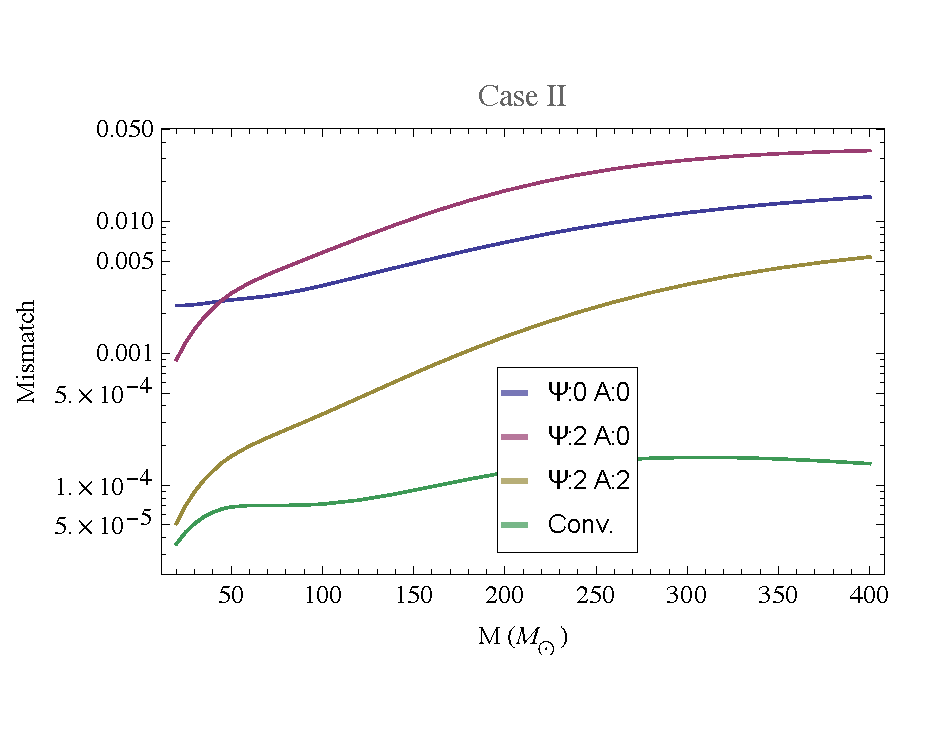
\includegraphics[width=.48\linewidth]{plots/precmmasympt.pdf}
  \caption{Mismatches computed between the exact FFT and the various approximations respresented in Figs.~\ref{fig:precerrorcaseI} and~\ref{fig:precerrorcaseII}.}
  \label{fig:precmm}
\end{figure}

%%%%%%%%%%%%%%%%%%%%%%%%%%%%%%%%%%%%
%%%%%%%%%%%%%%%%%%%%%%%%%%%%%%%%%%%%

\section{Summary and Conclusions}
\label{sec:conc}

[]

%%%%%%%%%%%%%%%%%%%%%%%%%%%%%%%%%%%%
%%%%%%%%%%%%%%%%%%%%%%%%%%%%%%%%%%%%

\vspace{4.5mm}

\hspace{0.85in}
{\bf Acknowledgments}

\vspace{3.5mm}

[Acknowledgments]

%%%%%%%%%%%%%%%%%%%%%%%%%%%%%%%%%%%%
%%%%%%%%%%%%%%%%%%%%%%%%%%%%%%%%%%%%

\appendix

\section{Appendix}
\label{app:}

%%%%%%%%%%%%%%%%%%%%%%%%%%%%%%%%%%%%
%%%%%%%%%%%%%%%%%%%%%%%%%%%%%%%%%%%%

%\bibliography{ListeRef.bib}
\bibliography{references.bib}


\end{document}

